% !Mode:: "TeX:UTF-8"
% Translator: Tianfan Fu: 12.1~12.3 Shenjian Zhao: 12.4~12.5
\chapter{应用}
\label{chap:applications}

在本章中,我们将介绍如何使用\gls{DL}来解决\gls{CV}、\gls{SR}、\gls{NLP}以及其他商业领域中的应用。
首先我们将讨论在许多最重要的\glssymbol{AI}应用中所需的大规模\gls{NN}的实现。
接着,我们将回顾\gls{DL}已经成功应用的几个特定领域。
尽管\gls{DL}的一个目标是设计能够处理各种任务的算法,然而截止目前\gls{DL}的应用仍然需要一定程度的特化。
例如,\gls{CV}中的任务对每一个样本都需要处理大量的输入特征(像素)。
\gls{NLP}任务的每一个输入特征都需要对大量的可能值(词汇表中的词)建模。
% 431

\section{大规模\glsentrytext{DL}}
\label{sec:large_scale_deep_learning}
% 431 

\gls{DL}的基本思想基于\gls{connectionism}:尽管\gls{ML}模型中单个生物性的神经元或者说是单个特征不是智能的,但是大量的神经元或者特征作用在一起往往能够表现出智能。
我们必须着重强调神经元数量必须\emph{很大}这个事实。
相比20世纪80年代,如今\gls{NN}的精度以及处理任务的复杂度都有一定提升,其中一个关键的因素就是网络规模的巨大提升
。
正如我们在\secref{sec:increasing_model_sizes}中看到的一样,在过去的三十年内,网络规模是以指数级的速度递增的。
然而如今的\gls{ANN}的规模也仅仅和昆虫的神经系统差不多。

由于规模的大小对于神经网络来说至关重要,因此深度学习需要高性能的硬件设施和软件实现。
%大规模\gls{NN}的必要性,所以\gls{DL}需要高性能的硬件设施和软件实现。
% 431

\subsection{快速的CPU实现}
\label{sec:fast_cpu_implementations}

传统的\gls{NN}是用单台机器的CPU来训练的。
如今,这种做法通常被视为是不可取的。
现在,我们通常使用\glssymbol{GPU}或者许多台机器的CPU连接在一起进行计算。
在使用这种昂贵配置之前,为论证CPU无法承担\gls{NN}所需的巨大计算量,研究者们付出了巨大的努力。
% 432 head


描述如何实现高效的数值CPU代码已经超出了本书的讨论范围,但是我们在这里还是要强调通过设计一些特定的CPU上的操作可以大大提升效率。
例如,在2011年,最好的CPU在训练\gls{NN}时使用\gls{fixed_point_arithmetic}能够比\gls{float_point_arithmetic}跑得更快。
通过调整\gls{fixed_point_arithmetic}的实现方式,\citet{Vanhoucke-et-al-2011}获得了3倍于一个强\gls{float_point_arithmetic}系统的速度。
% 相对一个很强的\gls{float_point_arithmetic}系统3倍的加速
因为各个新型CPU都有各自不同的特性,所以有时候采用\gls{float_point_arithmetic}实现会更快。
% 一条重要的准则就是通过特殊设计的数值运算可以获得巨大的回报。
一条重要的准则就是,通过特殊设计的数值运算,我们可以获得巨大的回报。
除了选择\gls{fixed_point_arithmetic}或者\gls{float_point_arithmetic}以外,其他的策略还包括了如通过优化数据结构避免高速缓存缺失、使用向量指令等。
%还包括其他的策略,如通过优化数据结构避免高速缓存缺失、使用向量指令等。
如果模型规模不会限制模型表现(不会影响模型精度)时,\gls{ML}的研究者们一般忽略这些实现的细节。
% 432

\subsection{GPU 实现}
\label{sec:gpu_implementations}

许多现代\gls{NN}的实现基于\firstall{GPU}。
\glsacr{GPU}最初是为图形应用而开发的专用硬件组件。
%是一种特殊设计的硬件,设计的原始目的是为了处理图形应用。
视频游戏系统的消费市场刺激了图形处理硬件的发展。
它为视频游戏所设计的特性也可以使\gls{NN}的计算受益。
% 432  

视频游戏的渲染要求许多操作能够快速并行地执行。
环境和角色模型通过一系列顶点的3D坐标确定。
为了将大量的3D坐标转化为2D显示器上的坐标,显卡必须并行地对许多顶点执行矩阵乘法与除法。
%显卡必须快速实现矩阵乘法或者除法。
之后,显卡必须并行地在每个像素上执行诸多计算,来确定每个像素点的颜色。
在这两种情况下,计算都是非常简单的,并且不涉及CPU通常遇到的复杂的分支运算。
例如,同一个刚体内的每个顶点都会乘上相同的矩阵;也就是说,不需要通过{\tt if}语句来判断确定每个顶点需要乘哪个矩阵。
各个计算过程之间也是完全相互独立的,因此能够实现并行操作。
计算过程还涉及处理大量内存缓冲以及描述每一个需要被渲染的对象的纹理(颜色模式)的位图信息。
总的来说,这使显卡设计为拥有高度并行特性以及很高的内存带宽,同时也付出了一些代价,如相比传统的CPU更慢的时钟速度以及更弱的处理分支运算的能力。
% p 433


与上述的实时图形算法相比,\gls{NN}算法所需要的性能特性是相同的。
\gls{NN}算法通常涉及大量参数、激活值、梯度值的缓冲区,其中每个值在每一次训练迭代中都要被完全更新。
这些缓冲太大,会超出传统的桌面计算机的高速缓存(cache),所以内存带宽通常会成为主要瓶颈。
相比CPU,\glssymbol{GPU}一个显著的优势是其极高的内存带宽。
\gls{NN}的训练算法通常并不涉及大量的分支运算与复杂的控制指令,所以更适合在\glssymbol{GPU}硬件上训练。
由于\gls{NN}能够被分为多个单独的``神经元'',并且独立于同一层内其他神经元进行处理,所以\gls{NN}可以从\glssymbol{GPU}的并行特性中受益匪浅。
% 433


\glssymbol{GPU}硬件最初专为图形任务而设计。
随着时间的推移,\glssymbol{GPU}也变得更灵活,允许定制的子程序处理转化顶点坐标或者计算像素颜色的任务。
原则上,\glssymbol{GPU}不要求这些像素值实际基于渲染任务。
只要将计算的输出值作为像素值写入缓冲区,\glssymbol{GPU}就可以用于科学计算。
\citet{Steinkrau2005}在GPU上实现了一个两层全连接的\gls{NN},并获得了相对基于CPU的基准方法三倍的加速。
不久以后,\citet{chellapilla:inria-00112631}也论证了相同的技术可以用来加速\gls{supervised}\gls{convolutional_network}的训练。
% 433


在\gls{GP_GPU}发布以后,使用显卡训练\gls{NN}的热度开始爆炸性地增长。
这种\gls{GP_GPU}可以执行任意的代码,而并非仅仅渲染子程序。
NVIDIA的CUDA编程语言使得我们可以用一种像C一样的语言实现任意代码。
由于相对简便的编程模型,强大的并行能力以及巨大的内存带宽,\gls{GP_GPU}为我们提供了训练\gls{NN}的理想平台。
在它发布以后不久,这个平台就迅速被\gls{DL}的研究者们所采纳~\citep{RainaICML09-small,Ciresan-2010}。



如何在\gls{GP_GPU}上写高效的代码依然是一个难题。
在\glssymbol{GPU}上获得良好表现所需的技术与CPU上的技术非常不同。
比如说,基于CPU的良好代码通常被设计为尽可能从高速缓存中读取更多的信息。
然而在\glssymbol{GPU}中,大多数可写内存位置并不会被高速缓存,所以计算某个值两次往往会比计算一次然后从内存中读取更快。
\glssymbol{GPU}代码是天生多线程的,不同线程之间必须仔细协调好。
例如,如果能够把数据\firstgls{coalesced}起来,那么涉及内存的操作一般会更快。
当几个线程同时需要读/写一个值时,像这样的\gls{coalesced}会作为一次内存操作出现。
不同的\glssymbol{GPU}可能采用不同的\gls{coalesced}读/写数据的方式。
通常来说,如果在$n$个线程中,线程$i$访问的是第$i+j$处的内存,其中$j$是$2$的某个幂的倍数,那么内存操作就易于\gls{coalesced}。
具体的设定在不同的\glssymbol{GPU}型号中有所区别。
\glssymbol{GPU}另一个常见的设定是使一个组中的所有线程都同时执行同一指令。
这意味着\glssymbol{GPU}难以执行分支操作。
线程被分为一个个称作\firstgls{warp}的小组。
在一个\gls{warp}中的每一个线程在每一个循环中执行同一指令,所以当同一个\gls{warp}中的不同线程需要执行不同的指令时,需要使用串行而非并行的方式。
% 434 


由于实现高效\glssymbol{GPU}代码的困难性,研究人员应该组织好他们的工作流程,避免对每一个新的模型或算法都编写新的\glssymbol{GPU}代码。
通常来讲,人们会选择建立一个包含高效操作(如卷积和矩阵乘法)的软件库解决这个问题,然后再从库中调用所需要的操作确定模型。
%例如,\gls{ML}库Pylearn2 \citep{pylearn2_arxiv_2013}通过调用Theano \citep{bergstra+al:2010-scipy-short,Bastien-2012}和cuda-convnet \citep{Krizhevsky2010tr}提供的高性能操作,囊括了许多\gls{ML}算法。
例如,\gls{ML}库Pylearn2 \citep{pylearn2_arxiv_2013}将其所有的\gls{ML}算法都通过调用Theano~\citep{bergstra+al:2010-scipy-short,Bastien-2012}和cuda-convnet~\citep{Krizhevsky2010tr} 所提供的高性能操作来指定。
这种分解方法还可以简化对多种硬件的支持。
例如,同一个Theano程序可以在CPU或者\glssymbol{GPU}上运行,而不需要改变调用Theano的方式。
其他库如Tensorflow\citep{tensorflow}和Torch\citep{Torch-2011}也提供了类似的功能。
% 434 end


\subsection{大规模的分布式实现}
\label{sec:large_scale_distributed_implementations}

在许多情况下,单个机器的计算资源是有限的。
因此,我们希望把训练或者推断的任务分摊到多个机器上进行。
% 434 end

分布式的推断是容易实现的,因为每一个输入的样本都可以在单独的机器上运行。
这也被称为\firstgls{data_parallelism}。

同样地,\firstgls{model_parallelism}也是可行的,其中多个机器共同运行一个数据点,每一个机器负责模型的一个部分。
对于推断和训练,这都是可行的。
% 435



在训练过程中,\gls{data_parallelism}某种程度上来说更加困难
对于\gls{SGD}的单步来说,我们可以增加\gls{minibatch}的大小,但是从优化性能的角度来说,我们得到的回报通常并不会线性增长。
使用多个机器并行地计算多个\gls{GD}步骤是一个更好的选择。
不幸的是,\gls{GD}的标准定义完全是一个串行的过程:
第$t$步的梯度是第$t-1$步所得参数的函数。
% 435


这个问题可以使用\firstgls{ASGD}\citep{Bengio+Bengio96,Recht-et-al-NIPS2011}解决。
在这个方法中,几个处理器的核共用存有参数的内存。
每一个核在无锁情况下读取这些参数并计算对应的梯度,然后在无锁状态下更新这些参数。
%这种方法减少了每一个\gls{GD}所获得的平均提升,因为一些核把其他的核所更新的参数(写)覆盖了。
由于一些核把其他的核所更新的参数覆盖了,因此这种方法减少了每一步\gls{GD}所获得的平均提升。
但因为更新步数的速率增加,总体上还是加快了学习过程。
\citet{Dean-et-al-NIPS2012}率先提出了多机器无锁的\gls{GD}方法,其中参数是由\firstgls{parameter_server}管理而非存储在共用的内存中。
分布式的异步\gls{GD}方法保留了训练\gls{DNN}的基本策略,并被工业界很多\gls{ML}组所使用\citep{chilimbi2014project,Wu-et-al-arXiv2015}。
学术界的\gls{DL}研究者们通常无法负担那么大规模的分布式学习系统,但是一些研究仍关注于如何在校园环境中使用相对廉价的硬件系统构造分布式网络~\citep{icml2013_coates13}。
% 435


\subsection{\glsentrytext{model_compression}}
\label{sec:model_compression}
% 435 

在许多商业应用的\gls{ML}模型中,一个时间和内存开销较小的推断算法比一个时间和内存开销较小的训练算法要更为重要。
对于那些不需要个性化设计的应用来说,我们只需要一次性的训练模型,然后它就可以被成千上万的用户使用。
在许多情况下,相比开发者,终端用户的可用资源往往更有限。
例如,开发者们可以使用巨大的计算机集群训练一个\gls{SR}的网络,然后将其部署到移动手机上。


减少推断所需开销的一个关键策略是\firstgls{model_compression}~\citep{bucilua2006model}。
\gls{model_compression}的基本思想是用一个更小的模型取代替原始耗时的模型,从而使得用来存储与评估所需的内存与运行时间更少。



当原始模型的规模很大,且我们需要防止\gls{overfitting}时,\gls{model_compression}就可以起到作用。
在许多情况下,拥有最小\gls{generalization}误差的模型往往是多个独立训练而成的模型的\gls{ensemble}。
评估所有$n$个\gls{ensemble}成员的成本很高。
有时候,当单个模型很大(例如,如果它使用\gls{dropout}正则化)时,其\gls{generalization}能力也会很好。
% 436 

这些巨大的模型能够学习到某个函数$f(\Vx)$,但选用的参数数量超过了任务所需的参数数量。
%仅仅训练样本数是有限的,所以网络的规模是受限的。
只是因为训练样本数是有限的,所以模型的规模才变得必要。
只要我们拟合了这个函数$f(\Vx)$,我们就可以通过将$f$作用于随机采样点$x$来生成有无穷多训练样本的训练集。
%我们就可以生成一个拥有了无穷多训练样本的训练集,只需将$f$作用于任意生成的$\Vx$。
然后,我们使用这些样本训练一个新的更小的模型,使其能够在这些点上拟合$f(\Vx)$。
为了更加充分地利用了这个新的小模型的\gls{capacity},最好从类似于真实测试数据(之后将提供给模型)的分布中采样$\Vx$。
这个过程可以通过损坏训练样本或者从原始训练数据训练的生成模型中采样完成。

此外,我们还可以仅在原始训练数据上训练一个更小的模型,但只是为了复制模型的其他特征,比如在不正确的类上的后验分布\citep{Hinton-dark-2014,hinton2015distilling}。
% 436 

\subsection{\glsentrytext{dynamic_structure}}
\label{sec:dynamic_structure}

一般来说,加速数据处理系统的一种策略是构造一个系统,这个系统用\firstgls{dynamic_structure}描述图中处理输入的所需计算过程。
在给定一个输入的情况中,数据处理系统可以动态地决定运行神经网络系统的哪一部分。
单个神经网络内部同样也存在\gls{dynamic_structure},给定输入信息,决定特征(\gls{hidden_unit})哪一部分用于计算。
这种神经网络中的\gls{dynamic_structure}有时被称为\firstgls{conditional_computation}\citep{bengio2013estimating,bengio-arxiv13-condcomp}。
由于模型结构许多部分可能只跟输入的一小部分有关,只计算那些需要的特征可以起到加速的目的。
% 436 

\gls{dynamic_structure}计算是一种基础的计算机科学方法,广泛应用于软件工程项目。
应用于神经网络的最简单的\gls{dynamic_structure}基于决定神经网络(或者其他\gls{ML}模型)中的哪些子集需要应用于特定的输入。
% 437 

在分类器中加速推断的可行策略是使用\firstgls{cascade}的分类器。
当目标是检测罕见对象(或事件)是否存在时,可以应用\gls{cascade}策略。
要确定对象是否存在,我们必须使用具有高\gls{capacity}、运行成本高的复杂分类器。 
然而,因为对象是罕见的,我们通常可以使用更少的计算拒绝不包含对象的输入。
在这些情况下,我们可以训练一序列分类器。
序列中的第一个分类器具有低\gls{capacity},训练为具有高\gls{recall}。
换句话说,他们被训练为确保对象存在时,我们不会错误地拒绝输入。
最后一个分类器被训练为具有高精度。
在测试时,我们按照顺序运行分类器进行推断,一旦\gls{cascade}中的任何一个拒绝它,就选择抛弃。
总的来说,这允许我们使用高\gls{capacity}模型以较高的置信度验证对象的存在,而不是强制我们为每个样本付出完全推断的成本。
有两种不同的方式可以使得\gls{cascade}实现高\gls{capacity}。
一种方法是使\gls{cascade}中靠后的成员单独具有高\gls{capacity}。
在这种情况下,由于系统中的一些个体成员具有高\gls{capacity},因此系统作为一个整体显然也具有高\gls{capacity}。
还可以使用另一种\gls{cascade},其中每个单独的模型具有低\gls{capacity},但是由于许多小型模型的组合,整个系统具有高\gls{capacity}。
\citet{Viola01}使用\gls{cascade}的增强\gls{decision_tree}实现了适合在手持数字相机中使用的快速并且鲁棒的面部检测器。
本质上,它们的分类器使用滑动窗口方法来定位面部。
分类器会检查许多的窗口,如果这些窗口内不包含面部则被拒绝。
\gls{cascade}的另一个版本使用早期模型来实现一种硬\gls{attention_mechanism}:\gls{cascade}的先遣成员定位对象,并且\gls{cascade}的后续成员在给定对象位置的情况下执行进一步处理。
例如,Google使用两步\gls{cascade}从街景视图图像中转换地址编号:首先使用一个\gls{ML}模型查找地址编号,然后使用另一个\gls{ML}模型将其转录\citep{Goodfellow+et+al-ICLR2014a}。
% 437 

\gls{decision_tree}本身是\gls{dynamic_structure}的一个例子,因为树中的每个节点决定应该使用哪个子树来评估输入。
一个结合\gls{DL}和\gls{dynamic_structure}的简单方法是训练一个\gls{decision_tree},其中每个节点使用神经网络做出决策\citep{guo1992classification},虽然这种方法没有实现加速推断计算的目标。
% 437 end



类似的,我们可以使用称为\firstgls{gater}的神经网络来选择在给定当前输入的情况下将使用几个\firstgls{expert_network}中的哪一个来计算输出。
这个想法的第一个版本被称为\firstgls{mixture_of_experts}\citep{Nowlan90,Jacobs-nc91},其中\gls{gater}为每个专家输出一个概率或权重(通过非线性的\gls{softmax}获得),并且最终输出由各个专家输出的加权组合获得。
在这种情况下,使用\gls{gater}不会降低计算成本,但如果每个样本的\gls{gater}选择单个专家,我们就会获得一个特殊的\firstgls{hard_mixture_of_experts}~\citep{collobert:2001:rr01-12,collobert:2002},这可以加速推断和训练。
当\gls{gater}决策的数量很小时,这个策略效果会很好,因为它不是组合的。
但是当我们想要选择不同的单元或参数子集时,不可能使用``软开关'',因为它需要枚举(和计算输出)所有的\gls{gater}配置。
为了解决这个问题,许多工作探索了几种方法来训练组合的\gls{gater}。
\citet{bengio-arxiv13-condcomp}提出使用\gls{gater}概率梯度的若干估计器,而\citet{Bacon-et-al-RLDM2015,BengioE-et-al-arXiv2015}使用\gls{RL}技术(\firstgls{policy_gradient})来学习一种条件的\gls{dropout}形式(作用于\gls{hidden_unit}块),减少了实际的计算成本,而不会对近似的质量产生负面影响。
% 438


另一种\gls{dynamic_structure}是开关,其中隐藏单元可以根据具体情况从不同单元接收输入。
这种动态路由方法可以理解为\firstgls{attention_mechanism} \citep{Olshausen1993}。
目前为止,硬性开关的使用在大规模应用中还没有被证明是有效的。
较为先进的方法一般采用对许多可能的输入使用加权平均,因此不能完全得到\gls{dynamic_structure}所带来的计算益处。
先进的\gls{attention_mechanism}将在\secref{sec:using_an_attention_mechanism_and_aligning_pieces_of_data}中描述。
% 438



使用动态结构化系统的主要障碍是由于系统针对不同输入的不同代码分支导致的并行度降低。
这意味着网络中只有很少的操作可以被描述为对样本\gls{minibatch}的矩阵乘法或批量卷积。
我们可以写更多的专用子程序,用不同的核对样本做卷积,或者通过不同的权重列来乘以设计矩阵的每一行。
不幸的是,这些专用的子程序难以高效地实现。
由于缺乏高速缓存的一致性,CPU实现会十分缓慢。
此外,由于缺乏\gls{coalesced}的内存操作以及\gls{warp}成员使用不同分支时需要串行化操作,\glssymbol{GPU}的实现也会很慢。
在一些情况下,我们可以通过将样本分成组,并且都采用相同的分支并且同时处理这些样本组的方式来缓解这些问题。
在离线环境中,这是最小化处理固定量样本所需时间的一项可接受的策略。
然而在实时系统中,样本必须连续处理,对工作负载进行分区可能会导致负载均衡问题。
例如,如果我们分配一台机器处理\gls{cascade}中的第一步,另一台机器处理\gls{cascade}中的最后一步,那么第一台机器将倾向于过载,最后一个机器倾向于欠载。
如果每个机器被分配以实现神经\gls{decision_tree}的不同节点,也会出现类似的问题。
% 439


\subsection{深度网络的专用硬件实现}
\label{sec:specialized_hardware_implementations_of_deep_networks}
%439

自从早期的神经网络研究以来,硬件设计者已经致力于可以加速\gls{NN}算法的训练和/或推断的专用硬件实现。
读者可以查看早期和更近的专用硬件深度网络的评论\citep{Lindsey+Lindblad-1994,Beiu-et-al-2003,Misra+Saha-2010}。
%439


不同形式的专用硬件\citep{Graf+Jackel-1989,Mead+Ismail-2012,Kim-et-al-2009,Pham-et-al-2012,Chen-et-al-IEEE2014,Chen-et-al-ACM2014}的研究已经持续了好几十年,比如\firstall{ASIC}的数字(基于数字的二进制表示),模拟\citep{Graf+Jackel-1989,Mead+Ismail-2012}(基于以电压或电流表示连续值的物理实现)和混合实现(组合数字和模拟组件)。
近年来更灵活的\firstall{FPGA}实现(其中电路的具体细节可以在制造完成后写入芯片)也得到了长足发展。
% 439 mid



虽然CPU和\glssymbol{GPU}上的软件实现通常使用32或64位的精度来表示浮点数,但是长期以来使用较低的精度在更短的时间内完成推断也是可行的\citep{Holt-et-al-1991,Holi+Hwang-1993,Presley-et-al-1994,Simard+Graf-NIPS1994,Wawrzynek-et-al-IEEE1996,Savich-et-al-2007}。
这已成为近年来更迫切的问题,因为\gls{DL}在工业产品中越来越受欢迎,并且由于更快的硬件产生的巨大影响已经通过\glssymbol{GPU}的使用得到了证明。
激励当前对深度网络专用硬件研究的另一个因素是单个CPU或\glssymbol{GPU}核心的进展速度已经减慢,并且最近计算速度的改进来自于核心的并行化(无论CPU还是\glssymbol{GPU})。
这与20世纪90年代的情况(上一个神经网络时代)的不同之处在于,\gls{NN}的硬件实现(从开始到芯片可用可能需要两年)跟不上快速进展和价格低廉的通用CPU的脚步。
因此,在针对诸如手机等低功率设备开发新的硬件设计,并且想要用于\gls{DL}的一般公众应用(例如,具有语音、\gls{CV}或自然语言功能的设施)等时,研究专用硬件能够进一步推动其发展。
% 440 head


最近对基于\gls{BP}\gls{NN}的低精度实现的工作\citep{Vanhoucke-et-al-2011,Courbariaux-et-al-ICLR2015workshop,Gupta-et-al-2015}表明,8和16位之间的精度足以满足使用或训练基于\gls{BP}的\gls{DNN}的要求。
显而易见的是,在训练期间需要比在推断时更高的精度,并且数字某些形式的动态定点表示能够减少每个数需要的存储空间。
传统的定点数被限制在了一个固定范围之内(其对应于浮点表示中的给定指数)。
而动态定点表示在一组数字 (例如一个层中的所有权重) 之间共享该范围。
使用定点代替浮点表示并且每个数使用较少的比特能够减少执行乘法所需的硬件表面积、功率需求和计算时间。
而乘法已经是使用或训练\gls{BP}的现代深度网络中要求最高的操作。



% 440 new
\section{\glsentrytext{CV}}
\label{sec:computer_vision}

一直以来,\gls{CV}就是\gls{DL}应用中几个最活跃的研究方向之一。
因为视觉是一个对人类以及许多动物毫不费力,但对计算机却充满挑战的任务\citep{ballard1983parallel}。
\gls{DL}中许多流行的标准基准任务包括\gls{object_recognition}以及光学字符识别。
% 440  


\gls{CV}是一个非常广阔的发展领域,其中包括多种多样的处理图片的方式以及应用方向。
\gls{CV}的应用广泛:从复现人类视觉能力(比如识别人脸)到创造全新的视觉能力。
举个后者的例子,近期一个新的\gls{CV}应用是从视频中可视物体的振动中识别相应的声波\citep{Davis2014VisualMic}。
大多数\gls{CV}领域的\gls{DL}研究未曾关注过这样一个奇异的应用,它扩展了图像的范围,而不是仅仅关注于\gls{AI}中较小的核心目标——复制人类的能力。
无论是报告图像中存在哪个物体,还是给图像中每个对象周围添加注释性的边框,
或从图像中转录符号序列,或给图像中的每个像素标记它所属对象的标识,
大多数\gls{CV}中的\gls{DL}往往用于\gls{object_recognition}或者某种形式的检测。
由于\gls{generative_model}已经是\gls{DL}研究的指导原则,因此还有大量图像合成工作使用了深度模型。
尽管图像合成(``\emph{无中生有}'')通常不包括在\gls{CV}内,但是能够进行图像合成的模型通常用于图像恢复,即修复图像中的缺陷或从图像中移除对象这样的\gls{CV}任务。
% 441 

\subsection{预处理}
\label{sec:preprocessing}
% 441 

由于原始输入往往以\gls{DL}架构难以表示的形式出现,许多应用领域需要复杂精细的预处理。
\gls{CV}通常只需要相对少的这种预处理。
图像应该被标准化,从而使得它们的像素都在相同并且合理的范围内,比如$[0,1]$或者$[-1,1]$。
将$[0,1]$中的图像与$[0,255]$中的图像混合通常会导致失败。
将图像格式化为具有相同的比例严格上说是唯一一种必要的预处理。
许多\gls{CV}架构需要标准尺寸的图像,因此必须裁剪或缩放图像以适应该尺寸。
然而,严格地说即使是这种重新调整比例的操作并不总是必要的。
一些卷积模型接受可变大小的输入并动态地调整它们的\gls{pooling}区域大小以保持输出大小恒定\citep{Waibel89b}。
其他卷积模型具有可变大小的输出,其尺寸随输入自动缩放,例如对图像中的每个像素进行\gls{denoise}或标注的模型\citep{Hadsell-RSS-07}。
% 441 

\gls{dataset_augmentation}可以被看作是一种只对训练集做预处理的方式。
\gls{dataset_augmentation}是减少大多数\gls{CV}模型\gls{generalization}误差的一种极好方法。
在测试时可用的一个相关想法是将同一输入的许多不同版本传给模型(例如,在稍微不同的位置处裁剪的相同图像),并且在模型的不同实例上决定模型的输出。
后一个想法可以被理解为集成方法,并且有助于减少\gls{generalization}误差。
% 441 

其他种类的预处理需要同时应用于训练集和测试集,其目的是将每个样本置于更规范的形式,以便减少模型需要考虑的变化量。
减少数据中的变化量既能够减少\gls{generalization}误差,也能够减小拟合训练集所需模型的大小。
更简单的任务可以通过更小的模型来解决,而更简单的解决方案\gls{generalization}能力一般更好。
这种类型的预处理通常被设计为去除输入数据中的某种可变性,这对于人工设计者来说是容易描述的,并且人工设计者能够保证不受到任务影响。
当使用大型数据集和大型模型训练时,这种预处理通常是不必要的,并且最好只是让模型学习哪些变化性应该保留。
例如,用于分类ImageNet的AlexNet系统仅具有一个预处理步骤:对每个像素减去训练样本的平均值\citep{Krizhevsky-2012}。
% 442 

\subsubsection{对比度归一化}
\label{sec:contrast_normalization}
% 442 


在许多任务中,对比度是能够安全移除的最为明显的变化源之一。
简单地说,对比度指的是图像中亮像素和暗像素之间差异的大小。
量化图像对比度有许多方式。
在\gls{DL}中,对比度通常指的是图像或图像区域中像素的\gls{standard_deviation}。
假设我们有一个张量表示的图像$\TSX \in\SetR^{r\times c\times 3}$,其中$\TEX_{i,j,1}$表示第$i$行第$j$列红色的强度,$\TEX_{i,j,2}$对应的是绿色的强度,$\TEX_{i,j,3}$对应的是蓝色的强度。
然后整个图像的对比度可以表示如下:
\begin{align}
\label{eqn:121}
\sqrt{\frac{1}{3rc}\sum_{i=1}^{r} \sum_{j=1}^{c}\sum_{k=1}^{3} (\TEX_{i,j,k} - \bar{\TSX} )^2},
\end{align}
其中$\bar{\TSX}$是整个图片的平均强度,满足
\begin{align}
\label{eqn:122}
 \bar{\TSX} =  \frac{1}{3rc}\sum_{i=1}^{r} \sum_{j=1}^{c}\sum_{k=1}^{3}\TEX_{i,j,k}.
\end{align}


\firstall{GCN}旨在通过从每个图像中减去其平均值,然后重新缩放其使得其像素上的\gls{standard_deviation}等于某个常数$s$来防止图像具有变化的对比度。
这种方法非常复杂,因为没有缩放因子可以改变零对比度图像(所有像素都具有相等强度的图像)的对比度。
具有非常低但非零对比度的图像通常几乎没有信息内容。
在这种情况下除以真实\gls{standard_deviation}通常仅能放大传感器噪声或压缩伪像。
这种现象启发我们引入一个小的正的\gls{regularization}参数$\lambda$来平衡估计的\gls{standard_deviation}。
或者,我们至少可以约束分母使其大于等于$\epsilon$。
给定一个输入图像$\TSX$,\gls{GCN}产生输出图像$\TSX'$,定义为
\begin{align}
\label{eqn:123}
\TEX'_{i,j,k} = s\frac{\TEX_{i,j,k} - \bar{\TEX}}{\max\{ \epsilon, \sqrt{ \lambda + {\frac{1}{3rc}\sum_{i=1}^{r}\sum_{j=1}^{c}\sum_{k=1}^{3}} (\TEX_{i,j,k} - \bar{\TEX} )^2} \}}.
\end{align}
% 442 end


从大图像中剪切感兴趣的对象所组成的数据集不可能包含任何强度几乎恒定的图像。
在这些情况下,通过设置$\lambda = 0$来忽略小分母问题是安全的,并且在非常罕见的情况下为了避免除以$0$,通过将$\epsilon$设置为一个非常小的值比如说$10^{-8}$。
这也是\citet{Goodfellow+al-arxiv-2013}在CIFAR-10数据集上所使用的方法。
随机剪裁的小图像更可能具有几乎恒定的强度,使得激进的\gls{regularization}更有用。
在处理从CIFAR-10数据中随机选择的小区域时,\citet{Coates2011}使用$\epsilon = 0, \lambda = 10$。
% 443

尺度参数$s$通常可以设置为$1$(如\citet{Coates2011}所采用的),或选择使所有样本上每个像素的\gls{standard_deviation}接近$1$(如\citet{Goodfellow+al-arxiv-2013}所采用的)。
% 443 mid


公式~\eqref{eqn:123}中的\gls{standard_deviation}仅仅是对图片$L^2$范数的重新缩放(假设图像的平均值已经被移除)。
我们更偏向于根据\gls{standard_deviation}而不是$L^2$范数来定义\glssymbol{GCN},因为\gls{standard_deviation}包括除以像素数量这一步,从而基于\gls{standard_deviation}的\glssymbol{GCN}能够使用与图像大小无关的固定的$s$。
然而,观察到$L^2$范数与\gls{standard_deviation}成比例,这符合我们的直觉。
我们可以把\glssymbol{GCN}理解成到球壳的一种映射。
\figref{fig:gcn_sphere_color}对此有所说明。
这可能是一个有用的属性,因为\gls{NN}往往更好地响应空间方向,而不是精确的位置。
响应相同方向上的多个距离需要具有共线权重向量但具有不同偏置的\gls{hidden_unit}。
这样的情况对于学习算法来说可能是困难的。
此外,许多浅层的图模型把多个分离的模式表示在一条线上会出现问题。
\glssymbol{GCN}采用一个样本一个方向\footnote{译者:所有样本相似的距离}而不是不同的方向和距离来避免这些问题。
% 444 head

\begin{figure}[!htb]
\ifOpenSource
\centerline{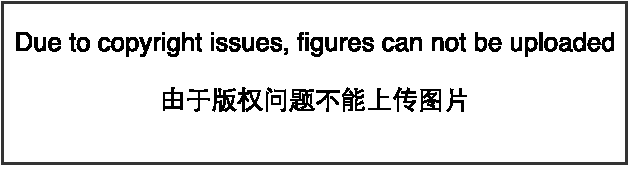
\includegraphics{figure.pdf}}
\else
	\centerline{\includegraphics{Chapter12/figures/gcn_sphere_color}}
\fi
	\caption{\glssymbol{GCN}将样本投影到一个球上。
\emph{(左)}原始的输入数据可能拥有任意的范数。
\emph{(中)}$\lambda=0$时候的\glssymbol{GCN}可以完美地将所有的非零样本投影到球上。
这里我们令$s=1$,$\epsilon = 10^{-8}$。
由于我们使用的\glssymbol{GCN}是基于归一化\gls{standard_deviation}而不是$L^2$范数,所得到的球并不是单位球。
\emph{(右)}$\lambda>0$的\gls{regularization}\glssymbol{GCN}将样本投影到球上,但是并没有完全地丢弃其范数中变化。
$s$和$\epsilon$的取值与之前一样。}
\label{fig:gcn_sphere_color}
\end{figure}
% 443 tail


% 444 head
与直觉相反的是,存在被称为\firstgls{sphering}的预处理操作,并且它不同于\glssymbol{GCN}。
\gls{sphering}并不会使数据位于球形壳上,而是将主成分重新缩放以具有相等方差,使得\glssymbol{PCA}使用的多变量正态分布具有球形等高线。 
\gls{sphering}通常被称为\firstgls{whitening}。
% 444 head


\gls{GCN}常常不能突出我们想要突出的图像特征,例如边缘和角。
如果我们有一个场景,包含了一个大的黑暗区域和一个大的明亮的区域(例如一个城市广场有一半的区域处于建筑物的阴影之中),
则\gls{GCN}将确保暗区域的亮度与亮区域的亮度之间存在大的差异。
然而,它不能确保暗区内的边缘突出。
% 444

这催生了\firstall{LCN} 。
\gls{LCN}确保对比度在每个小窗口上被归一化,而不是作为整体在图像上被归一化。
关于\gls{LCN}和\gls{GCN}的比较可以参考\figref{fig:122}。
% 444
% src0    gray0, gcn0?   lcn0  
%    src1?  gcn1?  gray1?     lcn1  
\begin{figure}[!htb]
\ifOpenSource
\centerline{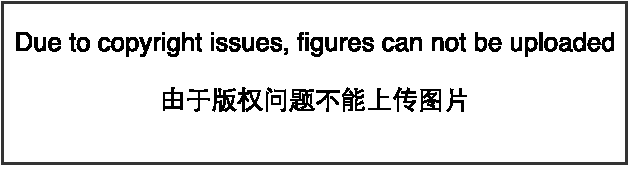
\includegraphics{figure.pdf}}
\else
    \centering
    \begin{tabular}{ccc}
        \includegraphics[width=.3\figwidth]{Chapter12/figures/src0.jpg} &
        \includegraphics[width=.3\figwidth]{Chapter12/figures/gcn0.jpg} &
        \includegraphics[width=.3\figwidth]{Chapter12/figures/lcn0.jpg} \\
        \includegraphics[width=.3\figwidth]{Chapter12/figures/src1.jpg} &   % ?? may be problem
        \includegraphics[width=.3\figwidth]{Chapter12/figures/gcn1.jpg} &
        \includegraphics[width=.3\figwidth]{Chapter12/figures/lcn1.jpg}\\
        Input image & GCN & LCN
    \end{tabular}
\fi
	\caption{\gls{GCN}和\gls{LCN}的比较。直观上说,\gls{GCN}的效果很巧妙。它使得所有的图片的尺度都差不多,这减轻了学习算法处理多个尺度的负担。\gls{LCN}更多地改变了图像,丢弃了所有相同强度的区域。这使得模型能够只关注于边缘。较好的纹理区域,如第二行的屋子,可能会由于归一化核的过高带宽而丢失一些细节。}
	\label{fig:122}
\end{figure}

\gls{LCN}的各种定义都是可行的。
在所有情况下,我们可以通过减去邻近像素的平均值并除以邻近像素的\gls{standard_deviation}来修改每个像素。
在一些情况下,要计算以当前要修改的像素为中心的矩形窗口中所有像素的平均值和\gls{standard_deviation}~\citep{Pinto08}。
在其他情况下,使用的则是以要修改的像素为中心的高斯权重的加权平均和加权\gls{standard_deviation}。
在彩色图像的情况下,一些策略单独处理不同的颜色通道,而其他策略组合来自不同通道的信息以使每个像素归一化\citep{sermanet-icpr-12}。
% 444

\gls{LCN}通常可以通过使用可分离卷积(参见\secref{sec:efficient_convolution_algorithms})来计算\gls{feature_map}的局部平均值和局部\gls{standard_deviation},然后在不同的\gls{feature_map}上使用逐元素的减法和除法。
% 444

\gls{LCN}是可微分的操作,并且还可以作为一种非线性作用应用于网络隐藏层,以及应用于输入的预处理操作。
% 444

与\gls{GCN}一样,我们通常需要\gls{regularization}\gls{LCN}来避免出现除以零的情况。
事实上,因为\gls{LCN}通常作用于较小的窗口,所以\gls{regularization}更加重要。
较小的窗口更可能包含彼此几乎相同的值,因此更可能具有零\gls{standard_deviation}。
% 445


\subsection{\glsentrytext{dataset_augmentation}}
\label{sec:dataset_augmentation_chap12}
如\secref{sec:dataset_augmentation_chap7}中讲到的一样,我们很容易通过增加训练集的额外副本来增加训练集的大小,进而改进分类器的\gls{generalization}能力。
这些额外副本可以通过对原始图像进行一些变化来生成,但是并不改变其类别。
\gls{object_recognition}这个分类任务特别适合于这种形式的\gls{dataset_augmentation},因为类别信息对于许多变换是不变的,而我们可以简单地对输入应用诸多几何变换。
如前所述,分类器可以受益于随机转换或者旋转,某些情况下输入的翻转可以增强数据集。
在专门的\gls{CV}应用中,存在很多更高级的用以\gls{dataset_augmentation}的变换。
这些方案包括图像中颜色的随机扰动~\citep{Krizhevsky-2012},以及对输入的非线性几何变形~\citep{chapter-gradient-document-2001}。
% 445




\section{\glsentrytext{SR}}
\label{sec:speech_recognition}
% 446

\gls{SR}任务在于将一段包括了自然语言发音的声学信号投影到对应说话人的词序列上。
令$\MX=(\Vx^{(1)},\Vx^{(2)},\ldots,\Vx^{(T)})$表示语音的输入向量(传统做法以$20$ms为一帧分割信号)。
许多\gls{SR}的系统通过特殊的手工设计方法预处理输入信号,从而提取特征,但是某些\gls{DL}系统\citep{jaitly2011learning}直接从原始输入中学习特征。
令$\Vy=(y_{1},y_{2},\ldots,y_{N})$表示目标的输出序列(通常是一个词或者字符的序列)。
\firstall{ASR}任务指的是构造一个函数$f^*_{\text{ASR}}$,使得它能够在给定声学序列$\MX$的情况下计算最有可能的语言序列$\Vy$:
\begin{align}
\label{eqn:124}
f^*_{\text{ASR}}(\MX) =  \underset{\Vy}{\arg\max}  P^*(\RVy \mid \RMX = \MX),
\end{align}
其中$P^*$是给定输入值$\MX$时对应目标$\Vy$的真实条件分布。
% 446

从20世纪80年代直到约2009-2012年,最先进的\gls{SR}系统是\firstall{HMM}和\firstall{GMM}的结合。
\glssymbol{GMM}对声学特征和\firstgls{phoneme}之间的关系建模\citep{Bahl87},\glssymbol{HMM}对\gls{phoneme}序列建模。
\glssymbol{GMM}-\glssymbol{HMM}模型将语音信号视作由如下过程生成:首先,一个\glssymbol{HMM}生成了一个\gls{phoneme}的序列以及离散的子\gls{phoneme}状态(比如每一个\gls{phoneme}的开始,中间,结尾),然后\glssymbol{GMM}把每一个离散的状态转化为一个简短的声音信号。
尽管直到最近\glssymbol{GMM}-\glssymbol{HMM}一直在\glssymbol{ASR}中占据主导地位,\gls{SR}仍然是\gls{NN}所成功应用的第一个领域。
从20世纪80年代末期到90年代初期,大量\gls{SR}系统使用了\gls{NN}\citep{Bourlard-cspla89,Waibel89b,Robinson+Fallside91,Bengio91z,Bengio92c,Konig96}。
当时,基于\gls{NN}的\glssymbol{ASR}的表现和\glssymbol{GMM}-\glssymbol{HMM}系统的表现差不多。
比如说,\citet{Robinson+Fallside91}在TIMIT数据集\citep{garofolo1993darpa}(有$39$个区分的\gls{phoneme}% ?? error
)上达到了$26$\%的\gls{phoneme}错误率,这个结果优于或者说是可以与基于\glssymbol{HMM}的结果相比。
从那时起,TIMIT成为了\gls{phoneme}识别的一个基准数据集,在\gls{SR}中的作用就和MNIST在\gls{object_recognition}中的作用差不多。
然而,由于\gls{SR}软件系统中复杂的工程因素以及在基于\glssymbol{GMM}-\glssymbol{HMM}的系统中已经付出的巨大努力,工业界并没有迫切转向\gls{NN}的需求。
结果,直到21世纪00年代末期,学术界和工业界的研究者们更多的是用\gls{NN}为\glssymbol{GMM}-\glssymbol{HMM}系统学习一些额外的特征。
% 447


之后,随着\emph{更大更深}的模型以及更大的数据集的出现,通过使用\gls{NN}代替\glssymbol{GMM}来实现将声学特征转化为\gls{phoneme}(或者子\gls{phoneme}状态)的过程可以大大地提高识别的精度。
从2009年开始,\gls{SR}的研究者们将一种\gls{unsupervised_learning}的\gls{DL}方法应用于\gls{SR}。
这种\gls{DL}方法基于训练一个被称作是\gls{RBM}的无向概率模型,从而对输入数据建模。
 \gls{RBM}将会在第三部分中描述。
 为了完成\gls{SR}任务,\gls{unsupervised}的\gls{pretraining}被用来构造一个\gls{deep_feedforward_network},这个\gls{NN}每一层都是通过训练\gls{RBM}来初始化的。
 这些网络的输入是从一个固定规格的输入窗(以当前帧为中心)的谱声学表示抽取,预测了当前帧所对应的\glssymbol{HMM}状态的条件概率。
 训练一个这样的\gls{NN}能够可以显著提高在TIMIT数据集上的识别率~\citep{mohamed2009deep,Mohamed+Dahl+Hinton-2012},并将\gls{phoneme}级别的错误率从大约$26$\%降到了$20.7$\%。
关于这个模型成功原因的详细分析可以参考\citet{mohamed2012understanding}。
对于基本的电话识别工作流程的一个扩展工作是添加说话人自适应相关特征\citep{mohamed2011deep}的方法,这可以进一步地降低错误率。
紧接着的工作则将结构从\gls{phoneme}识别(TIMIT所主要关注的)转向了大规模词汇语音识别\citep{Dahl2012},这不仅包含了识别\gls{phoneme},还包括了识别大规模词汇的序列。
\gls{SR}上的深度网络从最初的使用\gls{RBM}进行\gls{pretraining}发展到了使用诸如\gls{ReLU}和\gls{dropout}这样的技术~\citep{Zeiler+al-ICASSP-2013,Dahl-et-al-ICASSP2013}。
从那时开始,工业界的几个语音研究组开始寻求与学术圈的研究者之间的合作。
\citet{Hinton-et-al-2012}描述了这些合作所带来的突破性进展,这些技术现在被广泛应用在产品中,比如移动手机端。
% 447

随后,当研究组使用了越来越大的带标签的数据集,加入了各种初始化,训练方法以及调试\gls{DNN}的结构之后,
他们发现这种\gls{unsupervised}的\gls{pretraining}方式是没有必要的,或者说不能带来任何显著的改进。
% 447

用\gls{SR}中词错误率来衡量,在\gls{SR}性能上的这些突破是史无前例的(大约$30$\%的提高)。
在这之前的长达十年左右的时间内,尽管数据集的规模是随时间增长的(见\citet{Deng+Yu-2014}的图2.4),但基于\glssymbol{GMM}-\glssymbol{HMM}的系统的传统技术已经停滞不前了。
这也导致了\gls{SR}领域快速地转向\gls{DL}的研究。
在大约的两年时间内,工业界的大多数的\gls{SR}产品都包含了\gls{DNN},这种成功也激发了\glssymbol{ASR}领域对\gls{DL}算法和结构的一波新的研究浪潮,并且影响至今。
% 448

其中的一个创新点是\gls{convolutional_network}的应用~\citep{Sainath-et-al-ICASSP2013}。
\gls{convolutional_network}在时域与频域上复用了权重,改进了之前的仅在时域上使用重复权值的\gls{TDNNs}。
这种新的二维的卷积模型并不是将输入的频谱当作一个长的向量,而是当成是一个图像,其中一个轴对应着时间,另一个轴对应的是谱分量的频率。
% 448

完全抛弃\glssymbol{HMM}并转向研究\gls{end_to_end}\gls{DL}\gls{SR}系统是至今仍然活跃的另一个重要推动。
这个领域第一个主要的突破是\citet{Graves-et-al-ICASSP2013},其中训练了一个深度的\gls{LSTM}\gls{RNN}(见\secref{sec:the_long_short_term_memory_and_other_gated_rnns}),使用了帧-\gls{phoneme}排列的\glssymbol{MAP}推断,就像\citet{chapter-gradient-document-2001}以及CTC框架~\citep{Graves-et-al-2006,Graves-book2012}中一样。
一个深度\gls{RNN}~\citep{Graves-et-al-ICASSP2013}每个\gls{time_step}的各层都有状态变量,两种\gls{unfolded_graph}的方式导致两种不同深度:一种是普通的根据层的堆叠衡量的深度,另一种根据时间\gls{unfolding}衡量的深度。
这个工作把TIMIT数据集上\gls{phoneme}的错误率记录降到了的新低$17.7$\%。
关于应用于其他领域的深度\gls{RNN}的变种可以参考\citet{Pascanu-et-al-ICLR2014,Chung-et-al-NIPSDL2014-small}。
% 448

另一个\gls{end_to_end}\gls{DL}\gls{SR}方向的最新方法是让系统学习如何利用\firstgls{phonetic}层级的信息``排列''\firstgls{acoustic}层级的信息~\citep{Chorowski-et-al-arxiv2014,llu_is2015b}。
% 448


% Translator: Shenjian Zhao
\section{\glsentrytext{NLP}}
\label{sec: natural_language_processing}

\firstgls{NLP}让计算机能够使用人类语言,例如英语或法语。
为了让简单的程序能够高效明确地解析,计算机程序通常读取和发出特殊化的语言。
而自然的语言通常是模糊的,并且可能不遵循形式的描述。
\gls{NLP}中的应用如机器翻译,学习者需要读取一种人类语言的句子,并用另一种人类语言发出等同的句子。
许多\glssymbol{NLP}应用程序基于\gls{language_model},\gls{language_model}定义了关于自然语言中的字、字符或字节序列的概率分布。

% -- 448 --

与本章讨论的其他应用一样,非常通用的\gls{NN}技术可以成功地应用于\gls{NLP}。
然而,为了实现卓越的性能并扩展到大型应用程序,一些领域特定的策略也很重要。
为了构建自然语言的有效模型,通常必须使用专门处理序列数据的技术。
在很多情况下,我们将自然语言视为一系列词,而不是单个字符或字节序列。
因为可能的词总数非常大,基于词的\gls{language_model}必须在极高维度和稀疏的离散空间上操作。
为使这种空间上的模型在计算和统计意义上都高效,研究者已经开发了几种策略。

\subsection{\glsentrytext{n_gram}}
\label{sec:n_grams}

\firstgls{language_model}定义了自然语言中\gls{token}序列的概率分布。
根据模型的设计,\gls{token}可以是词、字符、甚至是字节。
\gls{token}总是离散的实体。
最早成功的\gls{language_model}基于固定长度序列的\gls{token}模型,称为\gls{n_gram}。
一个\gls{n_gram}是一个包含$n$个\gls{token}的序列。


基于\gls{n_gram}的模型定义一个条件概率——给定前$n-1$个\gls{token}后的第$n$个\gls{token}的条件概率。
该模型使用这些条件分布的乘积定义较长序列的概率分布:
\begin{align}
P(x_1, \dots, x_\tau) = P(x_1, \dots, x_{n-1}) \prod_{t=n}^\tau P(x_t \mid x_{t-n+1}, \dots, x_{t-1} ).
\end{align}
这个分解可以由概率的链式法则证明。
初始序列 $P(x_1, \dots, x_{n-1})$的概率分布可以通过带有较小$n$值的不同模型建模。

训练\gls{n_gram}模型是简单的,因为\gls{maximum_likelihood_estimation}可以通过简单地统计每个可能的\gls{n_gram}在训练集中出现的次数来获得。                                                                                                                                                                                                                                                                                                                                                                                       
几十年来,基于\gls{n_gram}的模型都是统计\gls{language_model}的核心模块~\citep{Jelinek+Mercer80,Katz87,Chen+Goodman99}。

对于小的$n$值,模型有特定的名称:$n=1$称为\firstgls{unigram},$n=2$称为\firstgls{bigram}及$n=3$称为\firstgls{trigram}。
这些名称源于相应数字的拉丁前缀和希腊后缀``-gram'',分别表示所写之物。

% -- 449 --

通常我们同时训练\gls{n_gram}模型和$n-1$ gram模型。 
这使得下式可以简单地通过查找两个存储的概率来计算。
\begin{align}
\label{eq:ml-ngram}
P(x_t \mid x_{t-n+1}, \dots, x_{t-1}) = \frac{P_n(x_{t-n+1}, \dots, x_t)} { P_{n-1}( x_{t-n+1}, \dots, x_{t-1}) }
\end{align}
为了在$P_n$中精确地再现\gls{inference},我们训练$P_{n-1}$时必须省略每个序列最后一个字符。

举个例子,我们演示三元模型如何计算句子``{\tt THE DOG RAN AWAY}.''的概率。
句子的第一个词不能通过上述条件概率的公式计算,因为句子的开头没有上下文。
取而代之,在句子的开头我们必须使用词的边缘概率。
因此我们计算$P_3({\tt THE\ DOG\ RAN})$。
最后,可以使用条件分布$P({\tt AWAY} \mid {\tt DOG\ RAN})$(典型情况)来预测最后一个词。
将这与式\eqref{eq:ml-ngram}放在一起,我们得到:
\begin{align}
P({\tt THE\ DOG\ RAN\ AWAY}) = P_3({\tt THE\ DOG\ RAN}) P_3({\tt DOG\ RAN\ AWAY}) / P_2({\tt DOG\ RAN}).
\end{align}

\gls{n_gram}模型最大似然的基本限制是,在许多情况下从训练集计数估计得到的$P_n$很可能为零(即使元组$(x_{t-n+1},  \dots, x_{t})$可能出现在测试集中)。
这可能会导致两种不同的灾难性后果。
当$P_{n-1}$为零时,该比率是未定义的,因此模型甚至不能产生有意义的输出。
当$P_{n-1}$非零而$P_n$为零时,测试样本的对数似然为 $-\infty$。
为避免这种灾难性的后果,大多数\gls{n_gram}模型采用某种形式的\firstgls{smoothing}。
\gls{smoothing}技术将概率质量从观察到的元组转移到类似的未观察到的元组。
见\citet{Chen+Goodman99}的综述和实验对比。
其中一种基本技术基于向所有可能的下一个符号值添加非零概率质量。
这个方法可以被证明是,计数参数具有均匀或\ENNAME{Dirichlet}先验的贝叶斯\gls{inference}。
另一个非常流行的想法是包含高阶和低阶\gls{n_gram}模型的混合模型,其中高阶模型提供更多的\gls{capacity},而低阶模型尽可能地避免零计数。
如果上下文$x_{t-n+k}, \ldots, x_{t-1}$的频率太小而不能使用高阶模型,\textbf{回退方法}(back-off methods)就查找低阶\gls{n_gram} 。
更正式地说,它们通过上下文$x_{t-n+k}, \ldots, x_{t-1}$估计$x_t$上的分布,并增加$k$直到找到足够可靠的估计。

% -- \450 --

经典的\gls{n_gram}模型特别容易引起\gls{curse_of_dimensionality}。
因为存在$|\SetV|^n$可能的\gls{n_gram},而且 $|\SetV|$ 通常很大。
即使有大量训练数据和适当的$n$,大多数\gls{n_gram}也不会出现在训练集中。
经典\gls{n_gram}模型的一种观点是执行最近邻查询。
换句话说,它可以被视为局部\gls{nonparametric}预测器,类似于$k$-最近邻。
这些极端局部预测器面临的统计问题已经在\secref{sec:local_constancy_and_smoothness_regularization}中描述过。
\gls{language_model}的问题甚至比普通模型更严重,因为任何两个不同的词在\gls{one_hot}向量空间中的距离彼此相同。
因此,难以大量利用来自任意``邻居''的信息 —— 只有重复相同上下文的训练样本对局部泛化有用。
为了克服这些问题,\gls{language_model}必须能够在一个词和其他语义相似的词之间共享知识。

为了提高\gls{n_gram}模型的统计效率,\textbf{基于类的语言模型}(class-based language model)~\citep{Brown92,Ney+Kneser93,Niesler98}引入词类别的概念,然后属于同一类别的词共享词之间的统计强度。
这个想法使用了聚类算法,基于它们与其他词同时出现的频率,将该组词分成集群或类。
随后,模型可以在条件竖杠的右侧使用词类ID而不是单个词ID。
混合(或回退)词模型和类模型的复合模型也是可能的。
尽管词类提供了在序列之间泛化的方式,但其中一些词被相同类的另一个替换,导致该\gls{representation}丢失了很多信息。

\subsection{\glsentrytext{NLM}}
\label{sec:neural_language_models}

\firstall{NLM}是一类用来克服\gls{curse_of_dimensionality}的\gls{language_model},它使用词的\gls{distributed_representation}对自然语言序列建模~\citep{BenDucVin01-small}。
不同于基于类的\gls{n_gram}模型,\gls{NLM}在能够识别两个相似的词,并且不丧失将每个词编码为彼此不同的能力。
\gls{NLM}共享一个词(及其上下文)和其他类似词(和上下文之间)的统计强度。
模型为每个词学习的\gls{distributed_representation},允许模型处理具有类似共同特征的词来实现这种共享。
例如,如果词{\tt dog}和词{\tt cat}映射到具有许多属性的表示,则包含词{\tt cat}的句子可以告知模型对包含词{\tt dog}的句子做出预测,反之亦然。
因为这样的属性很多,所以存在许多泛化的方式,可以将信息从每个训练语句传递到指数数量的语义相关语句。
\gls{curse_of_dimensionality}需要模型泛化到指数多的句子(指数相对句子长度而言)。
该模型通过将每个训练句子与指数数量的类似句子相关联克服这个问题。

% -- 451 --

我们有时将这些词\gls{representation}称为\firstgls{word_embedding}。
在这个解释下,我们将原始符号视为维度等于词表大小的空间中的点。
词\gls{representation}将这些点嵌入到较低维的特征空间中。
在原始空间中,每个词由一个\gls{one_hot}向量表示,因此每对词彼此之间的欧氏距离都是$\sqrt{2}$。
在嵌入空间中,经常出现在类似上下文(或共享由模型学习的一些``特征''的任何词对)中的词彼此接近。
这通常导致具有相似含义的词变得邻近。
\figref{fig:chap12_word_embeddings_color}放大了学到的\gls{word_embedding}空间的特定区域,我们可以看到语义上相似的词如何映射到彼此接近的表示。

\begin{figure}[htp]
\centering
\ifOpenSource
\centerline{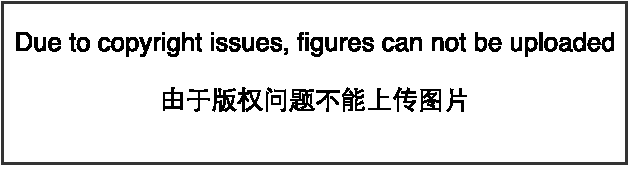
\includegraphics{figure.pdf}}
\else
\includegraphics{Chapter12/figures/word_embeddings_color.pdf}
\fi
\caption{从\gls{NMT}模型获得的\gls{word_embedding}的二维可视化\citep{Bahdanau-et-al-ICLR2015-small}。
此图在语义相关词的特定区域放大,它们具有彼此接近的嵌入向量。
国家在左图,数字在右图。
注意,这些嵌入是为了可视化才表示为2维。
在实际应用中,嵌入通常具有更高的维度并且可以同时捕获词之间多种相似性。
}
\label{fig:chap12_word_embeddings_color}
\end{figure}

其他领域的\gls{NN}也可以定义嵌入。
例如,\gls{convolutional_network}的隐藏层提供``图像嵌入''。
因为自然语言最初不在实值向量空间上,所以\glssymbol{NLP}从业者通常对嵌入的这个想法更感兴趣。
隐藏层在表示数据的方式上提供了更质变的戏剧性变化。

% -- 452 --

使用\gls{distributed_representation}来改进\gls{NLP}模型的基本思想不必局限于\gls{NN}。
它还可以用于\gls{graphical_model},其中\gls{distributed_representation}是多个\gls{latent_variable}的形式。

\subsection{高维输出}
\label{sec:high_dimensional_outputs}

在许多自然语言应用中,我们通常希望我们的模型产生词(而不是字符)作为输出的基本单位。
对于大词汇表,由于词汇量很大,在词的选择上表示输出分布的计算成本可能非常高。
在许多应用中,$\SetV$包含数十万词。
表示这种分布的朴素方法是应用一个仿射变换,将隐藏表示转换到输出空间,然后应用\ENNAME{softmax}函数。
假设我们的词汇表$\SetV$大小为$| \SetV |$。
因为其输出维数为$| \SetV |$,描述该仿射变换线性分量的权重矩阵非常大。
这造成了表示该矩阵的高存储成本,以及与之相乘的高计算成本。
因为\ENNAME{softmax}要在所有$| \SetV |$输出之间归一化,所以在训练时以及测试时执行全矩阵乘法是必要的 ——我们不能仅计算与正确输出的权重向量的点积。
因此,输出层的高计算成本在训练期间(计算似然性及其梯度)和测试期间(计算所有或所选词的概率)都有出现。
对于专门的\gls{loss_function},可以有效地计算梯度 \citep{Vincent2015},但是应用于传统\ENNAME{softmax}输出层的标准\gls{cross_entropy}损失时会出现许多困难。

假设$\Vh$是用于预测输出概率$\hat \Vy$的顶部隐藏层。
如果我们使用学到的权重$\MW$和学到的\gls{bias_aff} $\Vb$参数化从$\Vh$到$\hat \Vy$的变换,则仿射\ENNAME{softmax}输出层执行以下计算:
\begin{align}
\label{eq:softmax-over-words}
  a_i &= b_i + \sum_j  W_{ij} h_j \;\;\; \forall i \in \{1,\ldots,|\SetV|\}, \\
  \hat{y}_i &= \frac{e^{a_i}}{\sum_{i'=1}^{|\SetV|} e^{a_{i'}}}.
\end{align}
如果$\Vh$包含$n_h$个元素,则上述操作复杂度是 $O(|\SetV| n_h)$。
在$n_h$为数千和$| \SetV |$数十万的情况下,这个操作占据了\gls{NLM}的大多数计算。

% -- 453 --

\subsubsection{使用\glsentrytext{shortlist}}
第一个\gls{NLM}\citep{BenDucVin01-small,Bengio-nnlm2003-small}通过将词汇量限制为10,000或20,000来减轻大词汇表上\ENNAME{softmax}的高成本。
\citet{Schwenk+Gauvain2002}和 \citet{Schwenk-2007}在这种方法的基础上建立新的方式,将词汇表$\SetV$分为最常见词汇(由\gls{NN}处理)的\firstgls{shortlist}~$\SetL$和较稀有词汇的尾列表$\SetT = \SetV \backslash \SetL$(由\gls{n_gram}模型处理)。
为了组合这两个预测,\gls{NN}还必须预测在上下文$C$之后出现的词位于尾列表的概率。
我们可以添加额外的\ENNAME{sigmoid}输出单元估计 $P(i \in \SetT \mid C)$实现这个预测。
额外输出则可以用来估计$\SetV$中所有词的概率分布,如下:
\begin{align}
 P(y=i\mid C)  =& 1_{i \in \SetL} P(y=i\mid C, i \in \SetL) (1 - P(i \in \SetT\mid C)) \nonumber \\
     & + 1_{i \in \SetT} P(y=i\mid C, i \in \SetT) P(i \in \SetT\mid C),
\end{align}
其中$P(y=i\mid C, i \in \SetL)$由\gls{NLM}提供$P(y=i\mid C, i \in \SetT)$由\gls{n_gram}模型提供。
稍作修改,这种方法也可以在\gls{NLM}模型的\ENNAME{softmax}层中使用额外的输出值,而不是单独的\ENNAME{sigmoid}单元。

\gls{shortlist}方法的一个明显缺点是,\gls{NLM}的潜在泛化优势仅限于最常用的词,这大概是最没用的。
这个缺点引发了处理高维输出替代方法的探索,如下所述。

\subsubsection{分层Softmax}
减少大词汇表$\SetV$上高维输出层计算负担的经典方法~\citep{Goodman2001}是分层地分解概率。
$|\SetV|$因子可以降低到$\log |\SetV|$一样低,而无需执行与$|\SetV|$成比例数量(并且也与隐藏单元数量$n_h$成比例)的计算。
\citet{BengioTR1215}和\citet{Morin+Bengio-2005-small} 将这种因子分解方法引入\gls{NLM}中。

% -- 454 --

我们可以认为这种层次结构是先建立词的类别,然后是词类别的类别,然后是词类别的类别的类别等等。
这些嵌套类别构成一棵树,其叶子为词。
在平衡树中,树的深度为$\log |\SetV|$。
选择一个词的概率是由路径(从树根到包含该词叶子的路径)上的每个节点通向该词分支概率的乘积给出。
\figref{fig:chap12_word_hierarchy}是一个简单的例子。
\citet{Mnih+Hinton-2009}也描述了使用多个路径来识别单个词的方法,以便更好地建模具有多个含义的词。
计算词的概率则涉及在导向该词所有路径上的求和。
\begin{figure}[htp]
\centering
\ifOpenSource
\centerline{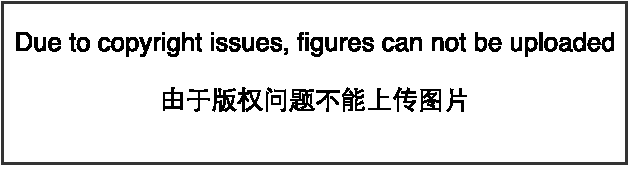
\includegraphics{figure.pdf}}
\else
\includegraphics{Chapter12/figures/word_hierarchy.pdf}
\fi
% Magic incantation to allow math in caption
\captionsetup{singlelinecheck=off}
% Part of the incantation is that we must define the [] argument
\caption[.]{词类别简单层次结构的示意图,其中8个词$w_0,\dots,w_7$组织成三级层次结构。
树的叶子表示实际特定的词。
内部节点表示词的组别。
任何节点都可以通过二值决策序列($0$=左,$1$=右)索引,从根到达节点。
超类$(0)$包含类$(0,0)$和$(0,1)$,其中分别包含词$\{w_0,w_1\}$和$\{w_2,w_3\}$的集合,类似地超类$(1)$包含类$(1,0)$和$(1,1)$,分别包含词$\{w_4,w_5\}$和$\{w_6,w_7\}$。
如果树充分平衡,则最大深度(二值决策的数量)与词数$| \SetV |$的对数同阶:从$| \SetV |$个词中选一个词只需执行$\CalO(\log |\SetV|)$次操作(从根开始的路径上的每个节点一次操作)。
在该示例中,我们乘三次概率就能计算词$y$的概率,这三次概率与从根到节点$y$的路径上每个节点向左或向右的二值决策相关联。
令$b_i(y)$为遍历树移向$y$时的第$i$个二值决策。
对输出$\RSy$进行采样的概率可以通过条件概率的链式法则分解为条件概率的乘积,其中每个节点由这些位的前缀索引。
例如,节点$(1,0)$对应于前缀$(b_0(w_4)=1, b_1(w_4)=0)$,并且$w_4$的概率可以如下分解:
\begin{align}
  P(\RSy = w_4) &= P(\RSb_0 = 1, \RSb_1 = 0, \RSb_2 = 0) \\
    &= P(\RSb_0 = 1) P(\RSb_1 = 0 \mid \RSb_0 = 1) P(\RSb_2 = 0 \mid \RSb_0 = 1, \RSb_1 = 0). 
\end{align}
}
\label{fig:chap12_word_hierarchy}
\end{figure}

为了预测树的每个节点所需的条件概率,我们通常在树的每个节点处使用\gls{logistic_regression}模型,并且为所有这些模型提供与输入相同的上下文$C$。
因为正确的输出编码在训练集中,我们可以使用\gls{supervised_learning}训练\gls{logistic_regression}模型。
我们通常使用标准\gls{cross_entropy}损失,对应于最大化正确判断序列的对数似然。

因为可以高效地计算输出对数似然(低至$\log |\SetV|$而不是$ |\SetV|$),所以也可以高效地计算梯度。
这不仅包括关于输出参数的梯度,而且还包括关于隐藏层激活的梯度。

优化树结构最小化期望的计算数量是可能的,但通常不切实际。
给定词的相对频率,信息理论的工具可以指定如何选择最佳的二进制编码。
为此,我们可以构造树,使得与词相关联的位数量近似等于该词频率的对数。
然而在实践中,节省计算通常事倍功半,因为输出概率的计算仅是\gls{NLM}中总计算的一部分。
例如,假设有$l$个全连接的宽度为$n_h$的隐藏层。
令$n_b$是识别一个词所需比特数的加权平均值,其加权由这些词的频率给出。
在这个例子中,计算隐藏激活所需的操作数增长为$O(ln_h^2)$,而输出计算增长为$O(n_h n_b)$。
只要$ n_b \leq l n_h$,我们可以通过收缩$n_h$比收缩$n_b$减少更多的计算量。
事实上,$n_b$通常很小。
因为词汇表的大小很少超过一百万而$\log_ 2(10^6) \approx 20$,所以可以将$n_b$减小到大约20,但$n_h$通常大得多,大约为$10^3$或更大。
我们可以定义深度为2和分支因子为$\sqrt{|\SetT|}$的树,而不用仔细优化分支因子为$2$的树。
这样的树对应于简单定义一组互斥的词类。
基于深度为$2$的树的简单方法可以获得层级策略大部分的计算益处。

% -- 455 --

一个仍然有点开放的问题是如何最好地定义这些词类,或者如何定义一般的词层次结构。
早期工作使用现有的层次结构\citep{Morin+Bengio-2005-small} ,但也可以理想地与\gls{NLM}联合学习层次结构。
学习层次结构很困难。
对数似然的精确优化似乎难以解决,因为词层次的选择是离散的,不适于基于梯度的优化。
然而,我们可以使用离散优化来近似地最优化词类的分割。

分层\ENNAME{softmax}的一个重要优点是,它在训练期间和测试期间(如果在测试时我们想计算特定词的概率)都带来了计算上的好处。

当然即使使用分层\ENNAME{softmax},计算所有$|\SetV|$个词概率的成本仍是很高的。
另一个重要的操作是在给定上下文中选择最可能的词。
不幸的是,树结构不能为这个问题提供高效精确的解决方案。

缺点是在实践中,分层\ENNAME{softmax}倾向于更差的测试结果(相对基于采样的方法),我们将在下文描述。
这可能是因为词类选择得不好。

\subsubsection{\glsentrytext{importance_sampling}}
\label{sec:importance_sampling_chap12}
加速\gls{NLM}训练的一种方式是,避免明确地计算所有未出现在下一位置的词对梯度的贡献。
每个不正确的词在此模型下具有低概率。
枚举所有这些词的计算成本可能会很高。
相反,我们可以仅采样词的子集。
使用式\eqref{eq:softmax-over-words}中引入的符号,梯度可以写成如下形式:
\begin{align}
 \frac{\partial \log P(y \mid C)}{\partial \theta} &= \frac{\partial \log {\rm softmax}_y(\Va)}{\partial \theta} \\ 
  &= \frac{\partial}{\partial \theta} \log \frac{e^{a_y}}{\sum_i e^{a_i}} \\ 
 &= \frac{\partial}{\partial \theta} (a_y - \log \sum_i e^{a_i}) \\ 
 &= \frac{\partial a_y}{\partial \theta}  - \sum_i P(y = i \mid C) \frac{\partial a_i}{\partial \theta},
\end{align}
其中$\Va$是\ENNAME{presoftmax}激活(或得分)向量,每个词对应一个元素。
第一项是\textbf{正相}(positive phase)项,推动$a_y$向上;而第二项是\textbf{负相}(negative phase)项,对于所有$i$以权重$P(i \mid C)$推动$a_i$向下。
由于负相项是期望值,我们可以通过\gls{monte_carlo}采样估计。
然而,这将需要从模型本身采样。
从模型中采样需要对词汇表中所有的$i$计算$P(i \mid C)$,这正是我们试图避免的。

我们可以从另一个分布中采样,而不是从模型中采样,这个分布称为\firstgls{proposal_distribution}(记为$q$),并通过适当的权重校正从错误分布采样引入的\gls{bias_sta} \citep{Bengio+Senecal-2003-small,Bengio+Senecal-2008}。
这是一种称为\firstgls{importance_sampling}的更通用技术的应用,我们将在\secref{sec:importance_sampling_chap12}中更详细地描述。
不幸的是,即使精确\gls{importance_sampling}也不一定有效,因为我们需要计算权重$p_i / q_i$,其中的$p_i = P(i \mid C)$只能在计算所有得分$a_i$后才能计算。
这个应用采取的解决方案称为\gls{biased_importance_sampling},其中重要性权重被归一化加和为1。
当对负词$n_i$进行采样时,相关联的梯度被加权为:
\begin{align}
  w_i = \frac{p_{n_i} / q_{n_i}}{\sum_{j=1}^N p_{n_j} / q_{n_j}}.
\end{align}
这些权重用于对来自$q$的$m$个负样本给出适当的重要性,以形成负相估计对梯度的贡献:
\begin{align}
  \sum_{i=1}^{|\SetV|} P(i \mid C) \frac{\partial a_i}{\partial \theta}  \approx \frac{1}{m} \sum_{i=1}^m w_i \frac{\partial a_{n_i}}{\partial \theta}.
  \end{align}
  \gls{unigram}或\gls{bigram}分布与\gls{proposal_distribution} $q$工作得一样好。
从数据估计这种分布的参数是很容易。
在估计参数之后,也可以非常高效地从这样的分布采样。

\firstgls{importance_sampling}不仅可以加速具有较大\ENNAME{softmax}输出的模型。
更一般地,它可以加速具有大稀疏输出层的训练,其中输出是稀疏向量而不是$n$选$1$。
其中一个例子是\firstgls{bag_of_words}。
\gls{bag_of_words}具有稀疏向量$\Vv$,其中$v_i$表示词汇表中的词$i$存不存在文档中。
或者,$v_i$可以指示词$i$出现的次数。
由于各种原因,训练产生这种稀疏向量的\gls{ML}模型的成本可能很高。
在学习的早期,模型可能不会真的使输出真正稀疏。
此外,将输出的每个元素与目标的每个元素进行比较,可能是描述训练的\gls{loss_function}最自然的方式。
这意味着稀疏输出并不一定能带来计算上的好处,因为模型可以选择使大多数输出非零,并且所有这些非零值需要与相应的训练目标进行比较( 即使训练目标是零)。
\citet{Dauphin2011-small} 证明可以使用\gls{importance_sampling}加速这种模型。
高效算法最小化``正词''(在目标中非零的那些词)和相等数量的``负词''的重构损失。
负词是被随机选取的,如使用启发式采样更可能被误解的词。
该启发式过采样引入的偏差则可以使用重要性权重校正。

% -- 458 --

在所有这些情况下,输出层梯度估计的计算复杂度被减少为与负样本数量成比例,而不是与输出向量的大小成比例。


\subsubsection{噪声对比估计和排名损失}


\label{sec:combining_neural_language_models_with_n_grams}
为减少训练大词汇表的\gls{NLM}的计算成本,研究者也提出了其他基于采样的方法。
早期的例子是 \citet{Collobert+Weston-ICML2008}提出的排名损失,将\gls{NLM}每个词的输出视为一个得分,并试图使正确词的得分$a_y$比其他词$a_i$排名更高。提出的排名损失则是
\begin{align} 
 L = \sum_i \max(0,1-a_y+a_i).
\end{align} 
如果观察到词的得分$a_y$远超过负词的得分$a_i$(相差大于1),则第$i$项梯度为零。
这个\gls{criterion}的一个问题是它不提供估计的条件概率,条件概率在很多应用中是有用的,包括语音识别和文本生成(包括诸如翻译的条件文本生成任务)。

最近用于\gls{NLM}的训练目标是噪声对比估计,将在\secref{sec:noise_contrastive_estimation}中介绍。
这种方法已成功应用于\gls{NLM}\citep{Mnih+Teh-ICML2012,Mnih2013}。

% -- 459 --

\subsection{结合\glsentrytext{n_gram}和\glsentrytext{NLM}}
\gls{n_gram}模型相对\gls{NN}的主要优点是\gls{n_gram}模型具有更高的模型\gls{capacity}(通过存储非常多的元组的频率),并且处理样本只需非常少的计算量(通过查找只匹配当前上下文的几个元组)。
如果我们使用哈希表或树来访问计数,那么用于\gls{n_gram}的计算量几乎与\gls{capacity}无关。
相比之下,将\gls{NN}的参数数目加倍通常也大致加倍计算时间。
当然,避免每次计算时使用所有参数的模型是一个例外。
嵌入层每次只索引单个嵌入,所以我们可以增加词汇量,而不会增加每个样本的计算时间。
一些其他模型,例如平铺\gls{convolutional_network},可以在减少\gls{parameter_sharing}程度的同时添加参数以保持相同的计算量。然而,基于矩阵乘法的典型\gls{NN}层需要与参数数量成比例的计算量。

因此,增加\gls{capacity}的一种简单方法是将两种方法结合,由\gls{NLM}和\gls{n_gram}\gls{language_model}组成\gls{ensemble}~\citep{BenDucVin01-small,Bengio-nnlm2003-small}。

对于任何\gls{ensemble},如果\gls{ensemble}成员产生独立的错误,这种技术可以减少测试误差。
\gls{ensemble}学习领域提供了许多方法来组合\gls{ensemble}成员的预测,包括统一加权和在验证集上选择权重。
\citet{Mikolov-Interspeech-2011} 扩展了\gls{ensemble},不是仅包括两个模型,而是包括大量模型。
我们也可以将\gls{NN}与最大熵模型配对并联合训练\citep{Mikolov-ASRU-2011}。
该方法可以被视为训练具有一组额外输入的\gls{NN},额外输入直接连接到输出并且不连接到模型的任何其他部分。
额外输入是输入上下文中特定\gls{n_gram}是否存在的指示器,因此这些变量是非常高维且非常稀疏的。

模型\gls{capacity}的增加是巨大的 (架构的新部分包含高达$| sV |^n$个参数 ),但是处理输入所需的额外计算量是很小的(因为额外输入非常稀疏)。

\subsection{\glsentrytext{NMT}}
\label{sec:neural_machine_translation}

机器翻译以一种自然语言读取句子并产生等同含义的另一种语言的句子。
机器翻译系统通常涉及许多组件。
在高层次,一个组件通常会提出许多候选翻译。
由于语言之间的差异,这些翻译中的许多翻译是不符合语法的。
例如,许多语言在名词后放置形容词,因此直接翻译成英语时,它们会产生诸如``apple red''的短语。
提议机制提出建议翻译的许多变体,理想情况下应包括``red apple''。
翻译系统的第二个组成部分(\gls{language_model})评估提议的翻译,并可以评估``red apple''比``apple red''更好。

% -- 460 --

最早的机器翻译\gls{NN}探索中已经纳入了\gls{encoder}和\gls{decoder}的想法(Allen 1987; Chrisman 1991; Forcada
and Ñeco 1997),而翻译中\gls{NN}的第一个大规模有竞争力的用途是通过\gls{NLM}升级翻译系统的\gls{language_model}~\citep{Schwenk-et-al-IWSLT2006,Schwenk-2010}。
之前,大多数机器翻译系统在该组件使用\gls{n_gram}模型。
机器翻译中基于\gls{n_gram}的模型不仅包括传统的回退\gls{n_gram}模型,而且包括\textbf{最大熵语言模型}(maximum entropy language models),其中给定上下文中常见的词,affine-softmax层预测下一个词。

传统\gls{language_model}仅仅报告自然语言句子的概率。
因为机器翻译涉及给定输入句子产生输出句子,所以将自然\gls{language_model}扩展为条件的是有意义的。
如\secref{sec:learning_conditional_distributions_with_maximum_likelihood}所述可以直接地扩展一个模型,该模型定义某些变量的边缘分布,以便在给定上下文$C$($C$可以是单个变量或变量列表)的情况下定义该变量的条件分布。
\citet{Devlin-et-al-ACL2014}在一些统计机器翻译的基准中击败了最先进的技术,他给定源语言中的短语$\RSs_1, \RSs_2,\ldots, \RSs_k$后使用\glssymbol{MLP}对目标语言的短语$\RSt_1, \RSt_2,\ldots, \RSt_k$进行评分。
这个\glssymbol{MLP}估计$P(\RSt_1, \RSt_2,\ldots, \RSt_k \mid \RSs_1, \RSs_2,\ldots, \RSs_k)$。
这个\glssymbol{MLP}的估计替代了条件\gls{n_gram}模型提供的估计。

基于\glssymbol{MLP}方法的缺点是需要将序列预处理为固定长度。
为了使翻译更加灵活,我们希望模型允许可变的输入长度和输出长度。
\glssymbol{RNN}具备这种能力。
\secref{sec:modeling_sequences_conditioned_on_context_with_rnns}描述了给定某些输入后,关于序列条件分布\glssymbol{RNN}的几种构造方法,并且\secref{sec:encoder_decoder_sequence_to_sequence_architectures}描述了当输入是序列时如何实现这种条件分布。
在所有情况下,一个模型首先读取输入序列并产生概括输入序列的数据结构。我们称这个概括为``上下文''$C$。
上下文$C$可以是向量列表,或者向量或张量。
读取输入以产生$C$的模型可以是\glssymbol{RNN}\citep{Cho-et-al-EMNLP2014,Sutskever-et-al-NIPS2014,Jean-et-al-arxiv2014}或\gls{convolutional_network}\citep{Kalchbrenner+Blunsom-EMNLP2013}。
另一个模型(通常是RNN),则读取上下文$C$并且生成目标语言的句子。
在\figref{fig:chap12_encoder_decoder_architecture}中展示了这种用于机器翻译的\gls{encoder}-\gls{decoder}框架的总体思想。

% -- 461 --

\begin{figure}[htp]
\ifOpenSource
\centerline{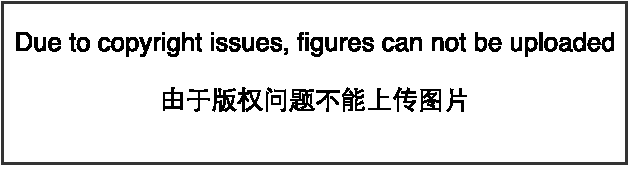
\includegraphics{figure.pdf}}
\else
\centerline{\includegraphics{Chapter12/figures/encoder_decoder_architecture.pdf}}
\fi
\caption{\gls{encoder}-\gls{decoder}架构在直观\gls{representation}(例如词序列或图像)和语义\gls{representation}之间来回映射。
使用来自一种模态数据的\gls{encoder}输出(例如从法语句子到捕获句子含义的隐藏\gls{representation}的\gls{encoder}映射)作为用于另一模态的\gls{decoder}输入(如\gls{decoder}将捕获句子含义的隐藏\gls{representation}映射到英语),我们可以训练将一种模态转换到另一种模态的系统。
这个想法已经成功应用于很多领域,不仅仅是机器翻译,还包括为图像生成标题。
}
\label{fig:chap12_encoder_decoder_architecture}
\end{figure}

为生成以源句为条件的整句,模型必须具有表示整个源句的方式。 
早期模型只能表示单个词或短语。
从\gls{representation_learning}的观点来看,具有相同含义的句子具有类似\gls{representation}是有用的,无论它们是以源语言还是以目标语言书写。
研究者首先使用卷积和\glssymbol{RNN}的组合探索该策略~\citep{Kalchbrenner+Blunsom-EMNLP2013}。
后来的工作介绍了使用\glssymbol{RNN}对所提议的翻译进行打分\citep{Cho-et-al-EMNLP2014}或生成翻译句子\citep{Sutskever-et-al-NIPS2014}。
\cite{Jean-et-al-arxiv2014}将这些模型扩展到更大的词汇表。

% -- 462 --

\subsubsection{使用\glsentrytext{attention_mechanism}并对齐数据片段}
\label{sec:using_an_attention_mechanism_and_aligning_pieces_of_data}
使用固定大小的表示概括非常长的句子(例如60个词)的所有语义细节是非常困难的。 
这需要使用足够大的RNN,并且用足够长时间训练得很好才能实现,如 \citet{Cho-et-al-EMNLP2014}和\citet{Sutskever-et-al-NIPS2014}所表明的。
然而,更高效的方法是先读取整个句子或段落(以获得正在表达的上下文和焦点),然后一次翻译一个词,每次聚焦于输入句子的不同部分来收集产生下一个输出词所需的语义细节。
这正是~\citet{Bahdanau-et-al-ICLR2015-small}第一次引入的想法。
\figref{fig:chap12_attention}中展示了\gls{attention_mechanism},其中每个\gls{time_step}关注输入序列的特定部分。

 \begin{figure}[htp]
\ifOpenSource
\centerline{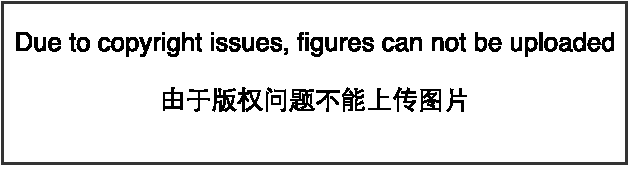
\includegraphics{figure.pdf}}
\else
\centerline{\includegraphics{Chapter12/figures/attention.pdf}}
\fi
\caption{由\citet{Bahdanau-et-al-ICLR2015-small}引入的现代\gls{attention_mechanism},本质上是加权平均。
\gls{attention_mechanism}对具有权重$\alpha^{(t)}$的特征向量$\Vh^{(t)}$进行加权平均形成上下文向量$\Vc$。
在一些应用中,特征向量$\Vh$是\gls{NN}的\gls{hidden_unit},但它们也可以是模型的原始输入。
权重$\alpha^{(t)}$由模型本身产生。
它们通常是区间$[0,1]$中的值,并且旨在仅仅集中在单个$\Vh^{(t)}$周围,使得加权平均精确地读取接近一个特定\gls{time_step}的特征向量。
权重$\alpha^{(t)}$通常由模型另一部分发出的相关性得分应用softmax函数后产生。
\gls{attention_mechanism}在计算上需要比直接索引期望的$\Vh^{(t)}$付出更高的代价,但直接索引不能使用\gls{GD}训练。
基于加权平均的\gls{attention_mechanism}是平滑、可微的近似,可以使用现有优化算法训练。
}
\label{fig:chap12_attention}
\end{figure}

我们可以认为基于\gls{attention_mechanism}的系统有三个组件:
\begin{itemize}
 \item   读取器\emph{读取}原始数据(例如源语句中的源词)并将其转换为\gls{distributed_representation},其中一个特征向量与每个词的位置相关联。
 \item 存储器存储读取器输出的特征向量列表。这可以被理解为包含事实序列的\emph{存储器},而之后不必以相同的顺序从中检索,也不必访问全部。
 \item 最后一个程序\emph{利用}存储器的内容顺序地执行任务,每个\gls{time_step}聚焦于某个存储器元素的内容(或几个,具有不同权重)。
\end{itemize}
第三组件可以生成翻译语句。

% -- 463 --

当用一种语言书写的句子中的词与另一种语言的翻译语句中的相应词对齐时,可以使对应的\gls{word_embedding}相关联。
早期的工作表明,我们可以学习将一种语言中的\gls{word_embedding}与另一种语言中的\gls{word_embedding}相关联的翻译矩阵\citep{Kocisky-et-al-ACL2014},与传统的基于短语表中频率计数的方法相比,可以产生较低的对齐错误率。
更早的工作\citep{Klementiev-et-al-COLING2012}也对跨语言词向量进行了研究。 
这种方法的存在很多扩展。
例如,允许在更大数据集上训练的更高效的跨语言对齐~\citep{Gouws-et-al-arxiv2014} 。

\subsection{历史展望}
\label{sec:historical_perspective_chap12}

在对\gls{back_propagation}的第一次探索中,\citet{Rumelhart86b-small}等人提出了\gls{distributed_representation}符号的思想,其中符号对应于族成员的身份,而\gls{NN}捕获族成员之间的关系,训练样本形成三元组如(Colin,Mother,Victoria)。
\gls{NN}的第一层学习每个族成员的表示。例如,Colin的特征可能代表Colin所在的族树,他所在树的分支,他来自哪一代等等。
我们可以将\gls{NN}认为是将这些属性关联在一起的计算学习规则,可以获得期望预测。
模型则可以进行预测,例如推断谁是Colin的母亲。

\cite{Deerwester90}将符号嵌入的想法扩展到对词的嵌入。
这些嵌入使用SVD学习。 
之后,嵌入将通过\gls{NN}学习。

\gls{NLP}的历史是由流行表示(对模型输入不同方式的表示)的变化为标志的。
在早期对符号和词建模的工作之后,\gls{NN}在\glssymbol{NLP}上一些最早的应用\citep{Miikkulainen91,Schmidhuber96}将输入表示为字符序列。

\citet{BenDucVin01-small} 将焦点重新引到对词建模并引入\gls{NLM},能产生可解释的\gls{word_embedding}。
这些神经模型已经从在一小组符号上的定义表示(20世纪80年代)扩展到现代应用中的数百万字(包括专有名词和拼写错误)。
这种计算扩展的努力导致了\secref{sec:high_dimensional_outputs}中描述的技术发明。

% -- 464 --

最初,使用词作为\gls{language_model}的基本单元可以改进语言建模的性能 \citep{BenDucVin01-small}。
而今,新技术不断推动基于字符 \citep{Sutskever-et-al-ICML2011})和基于词的模型向前发展,最近的工作 \citep{gillick2015multilingual}甚至建模Unicode字符的单个字节。

\gls{NLM}背后的思想已经扩展到多个\gls{NLP}应用,如解析\citep{Henderson-NAACL2003,Henderson-ACL2004,Collobert-AISTATS2011}、词性标注、语义角色标注、分块等,有时使用共享\gls{word_embedding}的单一多任务学习架构\citep{Collobert+Weston-ICML2008,collobert2011natural}。

随着t-SNE\gls{dimensionality_reduction}算法的发展\citep{VanDerMaaten08-small}以及Joseph Turian在2009年引入的专用于可视化词嵌入的应用,用于分析\gls{language_model}嵌入的二维可视化成为一种流行的工具。

\section{其他应用}
\label{sec:other_applications}

在本节中,我们介绍\gls{DL}一些其他类型的应用,它们与上面讨论的标准对象识别、语音识别和\gls{NLP}任务不同。
本书的第三部分将扩大这个范围,甚至进一步扩展到仍是目前主要研究领域的任务。


\subsection{\glsentrytext{recommender_system}}
\label{sec:recommender_systems}
信息技术部门中\gls{ML}的主要应用之一是向潜在用户或客户推荐项目。
这可以分为两种主要的应用:在线广告和项目建议(通常这些建议的目的仍然是为了销售产品)。
两者都依赖于预测用户和项目之间的关联, 一旦向该用户展示了广告或推荐了该产品,\gls{recommender_system}要么预测一些行为的概率(用户购买产品或该行为的一些代替)或预期增益(其可取决于产品的价值)。
目前,互联网的资金主要来自于各种形式的在线广告。
经济的主要部分依靠网上购物。 
包括Amazon和eBay在内的公司都使用了\gls{ML}(包括\gls{DL})推荐他们的产品。
有时,项目不是实际出售的产品。
如选择在社交网络新闻信息流上显示的帖子、推荐观看的电影、推荐笑话、推荐专家建议、匹配视频游戏的玩家或匹配约会的人。

% -- 465 --
通常,这种关联问题可以作为\gls{supervised_learning}问题来处理:给出一些关于项目和关于用户的信息,预测感兴趣的行为(用户点击广告、输入评级、点击``喜欢''按钮、 购买产品,在产品上花钱、花时间访问产品页面等)。
通常这最终会归结到回归问题(预测一些条件期望值)或概率分类问题(预测一些离散事件的条件概率)。

早期\gls{recommender_system}的工作依赖于这些预测输入的最小信息:用户ID和项目ID。
在这种情况下,唯一的泛化方式依赖于不同用户或不同项目的目标变量值之间的模式相似性。
假设用户1和用户2都喜欢项目A,B和C.
由此,我们可以推断出用户1和用户2具有类似的口味。
如果用户1喜欢项目D,那么这可以强烈提示用户2也喜欢D。
基于此原理的算法称为\firstgls{collaborative_filtering}。
非参数方法(例如基于估计偏好模式之间相似性的最近邻方法)和参数方法都可能用来解决这个问题。
参数方法通常依赖于为每个用户和每个项目学习\gls{distributed_representation}(也称为嵌入)。
目标变量的双线性预测(例如评级)是一种简单的参数方法,这种方法非常成功,通常被认为是最先进系统的组成部分。
通过用户嵌入和项目嵌入之间的点积(可能需要使用仅依赖于用户ID或项目ID的常数来校正)获得预测。
令$\hat{\MR}$是包含我们预测的矩阵,$\MA$矩阵行中是用户嵌入,$\MB$矩阵列中具有项目嵌入。
令$\Vb$和$\Vc$是分别包含针对每个用户(表示用户平常坏脾气或积极的程度)以及每个项目(表示其大体受欢迎程度)的\gls{bias_aff}向量。
因此,双线性预测如下获得:
\begin{equation}
\label{eq:bilinear-prediction}
 \hat{R}_{u,i} = b_u + c_i + \sum_j A_{u,j} B_{j,i}.
\end{equation}
通常,人们希望最小化预测评级$\hat{R}_{u,i}$ 和实际评级$\hat{R}_{u,i}$ 之间的平方误差。
当用户嵌入和项目嵌入首次缩小到低维度(两个或三个)时,它们就可以方便地可视化,或者可以将用户或项目彼此进行比较(就像\gls{word_embedding})。
获得这些嵌入的一种方式是对实际目标(例如评级)的矩阵$\MR$进行\gls{SVD}。
这对应于将$\MR = \MU \MD \MV'$(或归一化的变体)分解为两个因子的乘积,低秩矩阵 $\MA=\MU \MD$ and $\MB = \MV'$。
\glssymbol{SVD}的一个问题是它以任意方式处理缺失条目,如同它们对应于目标值0。
相反,我们希望避免为缺失条目做出的预测付出任何代价。
幸运的是,观察到的评级的平方误差总和也可以使用基于梯度的优化最小化。
\glssymbol{SVD}和式 \eqref{eq:bilinear-prediction}中的双线性预测在\ENNAME{Netflix}奖竞赛中(目的是仅基于大量匿名用户的之前评级预测电影的评级)表现得非常好\citep{bennett2007netflix}。
许多\gls{ML}专家参加了2006年和2009年之间的这场比赛。
它提高了使用先进\gls{ML}的\gls{recommender_system}的研究水平,并改进了\gls{recommender_system}。
即使简单的双线性预测或\glssymbol{SVD}本身并没有赢得比赛,但它是大多数竞争对手提出的整体模型中一个组成部分,包括胜者\citep{BigChaos-Netflix2009,Koren09}。

% -- 466 --

除了这些具有\gls{distributed_representation}的双线性模型之外,第一次用于\gls{collaborative_filtering}的\gls{NN}之一是基于\glssymbol{RBM}的无向概率模型~\citep{Salakhutdinov-2007-short}。
\glssymbol{RBM}是\ENNAME{Netflix}比赛获胜方法的一个重要组成部分\citep{BigChaos-Netflix2009,Koren09}。
\gls{NN}社群中也已经探索了对评级矩阵进行因子分解的更高级变体\citep{Salakhutdinov2008-small}。

然而,\gls{collaborative_filtering}系统有一个基本限制:当引入新项目或新用户时,缺乏评级历史意味着无法评估其与其他项目或用户的相似性,或者说无法评估新的用户和现有项目的联系。
这被称为冷启动推荐问题。
解决冷启动推荐问题的一般方式是引入单个用户和项目的额外信息。
例如,该额外信息可以是用户简要信息或每个项目的特征。
使用这种信息的系统被称为\textbf{基于内容的推荐系统}(content-based recommender system)。
从丰富的用户特征或项目特征集到嵌入的映射可以通过\gls{DL}架构学习\citep{Huang-et-al-2013,Elkahky-et-al-2015}。

专用的\gls{DL}架构,如\gls{convolutional_network}已经应用于从丰富内容中提取特征,如提取用于音乐推荐的音乐音轨\citep{vandenOord-et-al-NIPS2013}。
在该工作中,\gls{convolutional_network}将声学特征作为输入并计算相关歌曲的嵌入。
该歌曲嵌入和用户嵌入之间的点积则可以预测用户是否将收听该歌曲。

% -- 467 --

\subsubsection{\glsentrytext{exploration}与\glsentrytext{exploitation}}
当向用户推荐时,会产生超出普通\gls{supervised_learning}范围的问题,并进入\gls{RL}的领域。
理论上,许多推荐问题最准确的描述是\gls{contextual_bandit}\citep{Langford+Zhang-NIPS2008,Lu-et-al-2010}。
问题是,当我们使用\gls{recommender_system}收集数据时,我们得到是一个有偏且不完整的用户偏好观:我们只能看到用户对推荐给他们项目的反应,而不是其他项目。
此外,在某些情况下,我们可能无法获得未向其进行推荐的用户的任何信息(例如,在广告竞价中,可能是广告的建议价格低于最低价格阈值,或者没有赢得竞价,因此广告不会显示)。
更重要的是,我们不知道推荐任何其他项目会产生什么结果。
这就像训练一个分类器,为每个训练样本$\Vx$挑选一个类别$\hat y$(通常是基于模型最高概率的类别),然后只能获得该类别正确与否的反馈。
显然,每个样本传达的信息少于监督的情况(其中真实标签$y$是可直接访问的),因此需要更多的样本。
更糟糕的是,如果我们不够小心,即使收集越来越多的数据,我们得到的系统可能会继续选择错误的决定,因为正确的决定最初只有很低的概率:直到学习者选择正确的决定之前,该系统都无法学习正确的决定。
这类似于\gls{RL}的情况,其中仅观察到所选动作的奖励。
一般来说,\gls{RL}会涉及许多动作和许多奖励的序列。
\gls{bandit}情景是\gls{RL}的特殊情况,其中学习者仅采取单一动作并接收单个奖励。
\gls{bandit}问题在学习者知道哪个奖励与哪个动作相关联的时更容易。
在一般的\gls{RL}场景中,高奖励或低奖励可能是由最近的动作或很久以前的动作引起的。
术语\firstgls{contextual_bandit}指的是在一些输入变量可以通知决定的上下文中采取动作的情况。
例如,我们至少知道用户身份,并且我们要选择一个项目。
从上下文到动作的映射也称为\firstgls{policy}。
学习者和数据分布(现在取决于学习者的动作)之间的反馈循环是\gls{RL}和\gls{bandit}研究的中心问题。

% -- 468 --

\gls{RL}需要权衡\firstgls{exploration}与\firstgls{exploitation}。
\gls{exploitation}指的是从目前学到的最好\gls{policy}采取动作,也就是我们所知的将获得高奖励的动作。
\firstgls{exploration}是指采取行动以获得更多的训练数据。
如果我们知道给定上下文$\Vx$,动作$a$给予我们1的奖励,但我们不知道这是否是最好的奖励。
我们可能想利用我们目前的\gls{policy},并继续采取行动$a$相对肯定地获得1的奖励。
然而,我们也可能想通过尝试动作$a'$来探索。
我们不知道尝试动作$a'$会发生什么。
我们希望得到2的奖励,但有获得0奖励的风险。
无论如何,我们至少获得了一些知识。

\firstgls{exploration}可以以许多方式实现,从覆盖可能动作的整个空间的随机动作到基于模型的方法(基于预期回报和模型对该回报不确定性的量来计算动作的选择)。

许多因素决定了我们喜欢\gls{exploration}或\gls{exploitation}的程度。
最突出的因素之一是我们感兴趣的时间尺度。
如果代理只有短暂的时间积累奖励,那么我们喜欢更多的\gls{exploitation}。
如果代理有很长时间积累奖励,那么我们开始更多的\gls{exploration},以便使用更多的知识更有效地规划未来的动作。

\gls{supervised_learning}在\gls{exploration}或\gls{exploitation}之间没有权衡,因为监督信号总是指定哪个输出对于每个输入是正确的。
我们总是知道标签是最好的输出,没有必要尝试不同的输出来确定是否优于模型当前的输出 。

除了权衡\gls{exploration}和\gls{exploitation}之外,\gls{RL}背景下出现的另一个困难是难以评估和比较不同的\gls{policy}。
\gls{RL}包括学习者和环境之间的相互作用。
这个反馈回路意味着使用固定的测试集输入评估学习者的表现不是直接的。
\gls{policy}本身确定将看到哪些输入。
\citet{Dudik-2011} 提出了评估\gls{contextual_bandit}的技术。

% -- 469 --

\subsection{知识表示、推理和回答}
\label{sec:knowledge_representation_reasoning and_question_answering}
因为使用符号\citep{Rumelhart86b-small}和词嵌入\citep{Deerwester90,BenDucVin01-small},\gls{DL}方法在\gls{language_model}、机器翻译和\gls{NLP}方面非常成功。
这些嵌入表示关于单个词或概念的语义知识。
研究前沿是为短语或词和事实之间的关系开发嵌入。
搜索引擎已经使用\gls{ML}来实现这一目的,但是要改进这些更高级的表示还有许多工作要做。

\subsubsection{知识、联系和回答}
一个有趣的研究方向是确定如何训练\gls{distributed_representation}才能捕获两个实体之间的\firstgls{relation}。

数学中,\gls{binary_relation}是一组有序的对象对。
集合中的对具有这种关系,而那些不在集合中的对则没有。
例如,我们可以在实体集$\{ 1, 2, 3 \}$上定义关系``小于''来定义有序对的集合$\SetS = \{ (1, 2), (1, 3), (2, 3) \}$。
一旦这个关系被定义,我们可以像动词一样使用它。
因为$(1, 2) \in \SetS$,我们说1小于2。
因为$(2, 1) \not \in \SetS$,我们不能说2小于1。
当然,彼此相关的实体不必是数字。
我们可以定义关系{\tt is\_a\_type\_of}包含如{\tt(狗,哺乳动物)}的元组。

在\glssymbol{AI}的背景下,我们将\gls{relation}看作句法上简单且高度结构化的语言。
\gls{relation}起到动词的作用,而\gls{relation}的两个参数发挥着主体和客体的作用。
这些句子是一个三元组\gls{token}的形式:
\begin{align}
({\rm subject}, {\rm verb}, {\rm object})
\end{align}
其值是
\begin{align}
  ({\rm entity}_i, {\rm relation}_j, {\rm entity}_k).
\end{align}

我们还可以定义\firstgls{attribute},类似于\gls{relation}的概念,但只需要一个参数:
\begin{align}
  ( {\rm entity}_i, {\rm attribute}_j ).
\end{align}
例如,我们可以定义{\tt has\_fur} 属性,并将其应用于像{\tt 狗}这样的实体。

许多应用中需要表示\gls{relation}和推理。
我们如何在\gls{NN}中做到这一点?

\gls{ML}模型当然需要训练数据。
我们可以推断非结构化自然语言组成的训练数据集中实体之间的\gls{relation},也可以使用明确定义\gls{relation}的结构化数据库。 
这些数据库的共同结构是\gls{relational_database},它存储这种相同类型的信息,虽然没有格式化为三元\gls{token}的句子。
当数据库旨在将日常生活中常识或关于应用领域的专业知识传达给\gls{AI}系统时,我们将这种数据库称为\gls{knowledge_base}。
\gls{knowledge_base}包括一般的像{\tt Freebase}、{\tt OpenCyc}、 {\tt WordNet}、 {\tt Wikibase}\footnote{分别可以在如下网址获取: \url{freebase.com}, \url{cyc.com/opencyc},
\url{wordnet.princeton.edu}, \url{wikiba.se}}等等,和专业的知识库,如GeneOntology\footnote{\url{geneontology.org}}。
实体和\gls{relation}的\gls{representation}可以将\gls{knowledge_base}中的每个三元组作为训练样本来学习,并且以最大化捕获它们的联合分布为训练目标\citep{Bordes-et-al-LSML2013}。

除了训练数据,我们还需定义训练的模型族。
一种常见的方法是将\gls{NLM}扩展到模型实体和\gls{relation}。
\gls{NLM}学习提供每个词\gls{distributed_representation}的向量。
他们还通过学习这些向量的函数来学习词之间的相互作用,例如哪些词可能出现在词序列之后。
我们可以学习每个关系的嵌入向量将这种方法扩展到实体和\gls{relation}。
事实上,建模语言和通过\gls{relation}编码建模知识的联系非常接近,研究人员可以\emph{同时}使用\gls{knowledge_base}\emph{和}自然语言句子训练这样的实体表示\citep{bordes-aaai-2011,Bordes-et-al-AISTATS2012-small,Wang-et-al-EMNLP2014},或组合来自多个\gls{relational_database}的数据~\citep{Bordes-et-al-NIPS2013}。
可能与这种模型相关联的特定参数化有许多种。
早期关于学习实体间\gls{relation}的工作~\citep{Paccanaro2000}假定高度受限的参数形式(``线性关系嵌入''),通常对\gls{relation}使用与实体形式不同的表示。
例如,\citet{Paccanaro2000}和\citet{bordes-aaai-2011} 用向量表示实体而矩阵表示\gls{relation},其思想是\gls{relation}在实体上相当于运算符。
或者,关系可以被认为是任何其他实体\citep{Bordes-et-al-AISTATS2012-small},允许我们关于关系作声明,但是更灵活的是将它们结合在一起并建模联合分布的机制。

这种模型的实际短期应用是\firstgls{link_prediction}:预测\gls{knowledge_graph}中缺失的弧。
这是基于旧事实推广新事实的一种形式。
目前存在的大多数\gls{knowledge_base}都是通过人力劳动构建的,这往往使\gls{knowledge_base}缺失许多并且可能是大多数真正的关系。
请查看\citet{Wang-et-al-AAAI2014}、\citet{Lin-et-al-AAAI2015}和\citet{Garcia-Duran-et-al-arxiv2015}中这样应用的例子。

我们很难评估\gls{link_prediction}任务上模型的性能,因为我们的数据集只有正样本(已知是真实的事实)。
如果模型提出了不在数据集中的事实,我们不确定模型是犯了错误还是发现了一个新的以前未知的事实。
度量基于测试模型如何将已知真实事实的留存集合与不太可能为真的其他事实相比较,因此有些不精确。
构造感兴趣的负样本(可能为假的事实)的常见方式是从真实事实开始,并创建该事实的损坏版本,例如用随机选择的不同实体替换\gls{relation}中的一个实体 。
通用的测试精度(10$\%$度量)计算模型在该事实的所有损坏版本的前10$\%$中选择``正确''事实的次数。

\gls{knowledge_base}和\gls{distributed_representation}的另一个应用是\firstgls{word_sense_disambiguation} \citep{Navigli+Verlardi-2005,Bordes-et-al-AISTATS2012-small},这个任务决定在某些语境中哪个词的意义是恰当。

最后,知识的\gls{relation}结合一个推理过程和对自然语言的理解可以让我们建立一个一般的问答系统。
一般的问答系统必须能处理输入信息并记住重要的事实,并以之后能检索和推理的方式组织。
这仍然是一个困难的开放性问题,只能在受限的``玩具''环境下解决。
目前,记住和检索特定声明性事实的最佳方法是使用显式记忆机制,如\secref{sec:explicit_memory}所述。
\gls{memory_network}最开始是被用来解决一个玩具问答任务\citep{Weston2014}。
\citet{Kumar-et-al-arxiv2015} 提出了一种扩展,使用GRU\gls{recurrent_network}将输入读入存储器并且在给定存储器的内容后产生回答。

\gls{DL}已经应用于其他许多应用(除了这里描述的应用以外),并且肯定会在此之后应用于更多的场景。
我们不可能全面描述与此主题相关的所有应用 。
本项调查尽可能地提供了在本文写作之时的代表性样本

第二部分介绍了涉及\gls{DL}的现代实践,包括了所有非常成功的方法。
一般而言,这些方法使用\gls{cost_function}的梯度寻找模型(近似于某些所期望的函数)的参数。
当具有足够的训练数据时,这种方法是非常强大的。
我们现在转到第三部分,开始进入研究领域,旨在使用较少的训练数据或执行更多样的任务。
而且相比目前为止所描述的情况,其中的挑战更困难并且远远没有解决。
